\chapter{Current Advances} 
\sffamily
\label{chap:Literature_Review}
%%%%%%%%%%%%%%%%%%%%%%%%%%%%%%%%%%%%

This report is a representation of the progress that has been made by the Aerodynamic Test Platform and Wings team during the 2025-2026 academic year. As stated in the summary of this report, the breakdown of this teams structure does not follow one main result, rather it encompasses three. While each subsection within the team is focused on the analysis of flapping forces, the progress of each is discussed separately.

\indent For the Aerodynamic Test Platform (ATP), Stan and Kevin have taken this year to solidify its use as a tool for other teams within the MFWF project. The prototype that was received at the start of the year was required a redesign to initialize testing. Through the iterative testing process, the platform was modified in its structure and electronics to support the fine resolution required for capturing the small forces produced by the MFWF. One of these redesigns involved the removal of the tension cable method of attaching the inner frame to the load cells. The large amount of compensation needed to sustain it was concluded to be unnecessary for the ATP's purpose. A successful redesign involved the use of rigid links to replace the tension cables, resulting in consistent force measurement without the need for compensation, but resulted in higher visibility of the force coupling effect on the 6-axis design. The platform was validated through a series of tests using the flapping actuators available, confirming its ability to be used as a tool for measuring qualitative differences in lift production. In-depth advances can be found in sections \ref{chap:Stan_Melchers} and \ref{chap:Kevin_Fair}.

\indent For the ATP neural network, Wade and Aidan have taken on the newly assigned responsibilities to learn about and apply machine learning to the Aerodynamic Test Platform (ATP) of the MFWF. For the Fall 2025 semester, the focus was on developing an understanding of the fundamental principles, methods, and applications of machine learning and applying this knowledge, utilizing NACA airfoil data to synthesize and validate two separate aerodynamic models as a preliminary exercise. For Wade and Aidan's in-depth advances, see sections \ref{chap:Wade_Schnurr} and \ref{chap:Aidan_Sheridan}, respectively.

\indent As for the MFWF's wings, Abdulrahman and Justin took significant steps in designing and characterizing new functional wings for the flyer. Using the final selected wing design in 22/23 as the baseline, the goal this year is to design and manufacture more wing design prototypes and expand our wing test database and the design iteration process by including dynamic testing. The results would then be used to select the final functional pair of wings. Abdulrahman, at the start of the project, focused on a comprehensive review of published literature to define the deformation and camber that maximizes the lift generation and efficiency of the flapping wing. The second part of the semester was focused on the designing and manufacturing of new wing prototypes. Justin focused on establishing the dynamic testing process, including the tracking setup and preliminary deformation measurements to support future wing comparisons. For in-depth advances by Abdul and Justin, see sections \ref{chap:Abdulrahman_Sirajudeen-Sanni} and \ref{chap:Justin_Denneny}, respectfully.

\newpage
\section{Mechanical Design of the ATP}
\label{chap:Stan_Melchers}
\textbf{Student:} Stan Melchers
\subsection{Background}
The previous year decided to create a new design of the Aerodynamics Test Platform (ATP) from scratch. They preformed various computer simulations including Finite Element Analysis (FEA) for manufactured components and testing of various designs within MSC Adams to determine which would be the most stable under the oscillations induced by the flapper. Below is an image of the final ATP design CAD model.

\begin{figure}[htb]
  \centering
  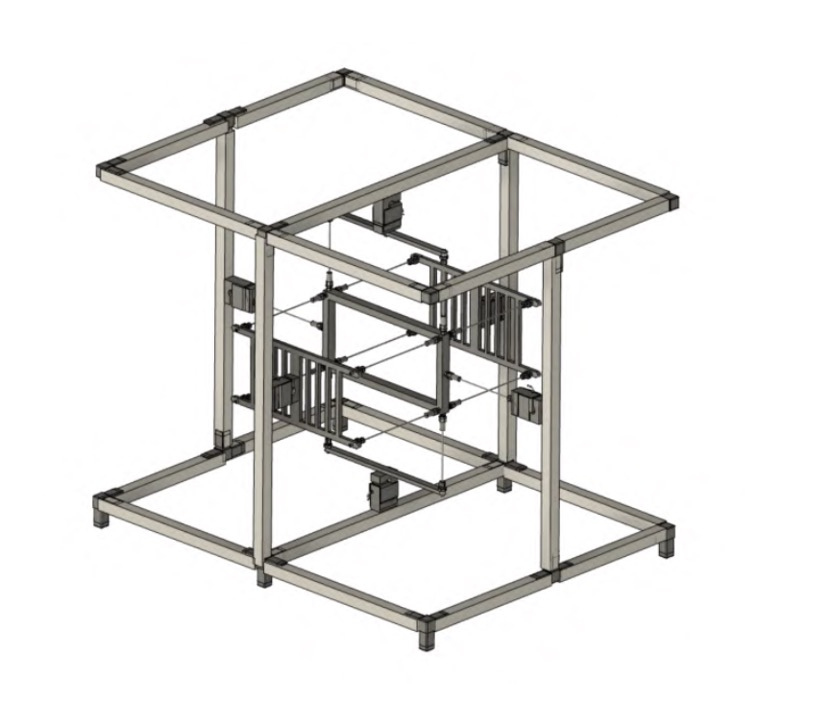
\includegraphics[height=6.5cm]{figures/Previous Year's ATP Design.jpg}
  \caption{Previous Year's ATP Design.}
  \label{fig:Previous_ATP_Design}
\end{figure}

The design consists of an outer frame made from aluminum extrusion and plastic press fit connectors. The base of the load cells are secured to the outer frame, the active end of the load cells are connected to crossbars using barrel adjusters and eight inch steel cables. There are six load cells within the design, two in each axis of motion. The crossbars are connected to the inner frame using more barrel adjusters and eight inch steel cables.

The previous year's team completed this design and was able to assemble the outer frame and some of the crossbars and cables. However, due to shipping timelines they were unable to assemble the entire design and begin testing.

In their handover letter, the previous year's team recommended the design of the inner frame be re-evaluated to better integrate with the flapper as well as the steel wire attachment mechanism between the inner frame and crossbars.

\subsection{Taking Stock of the Previous ATP Design}

The semester began by reviewing the previous year's progress on the ATP, and getting my hands on the ATP. Below is an image of the state of the ATP at the start of the year.

\begin{figure}[htb]
  \centering
  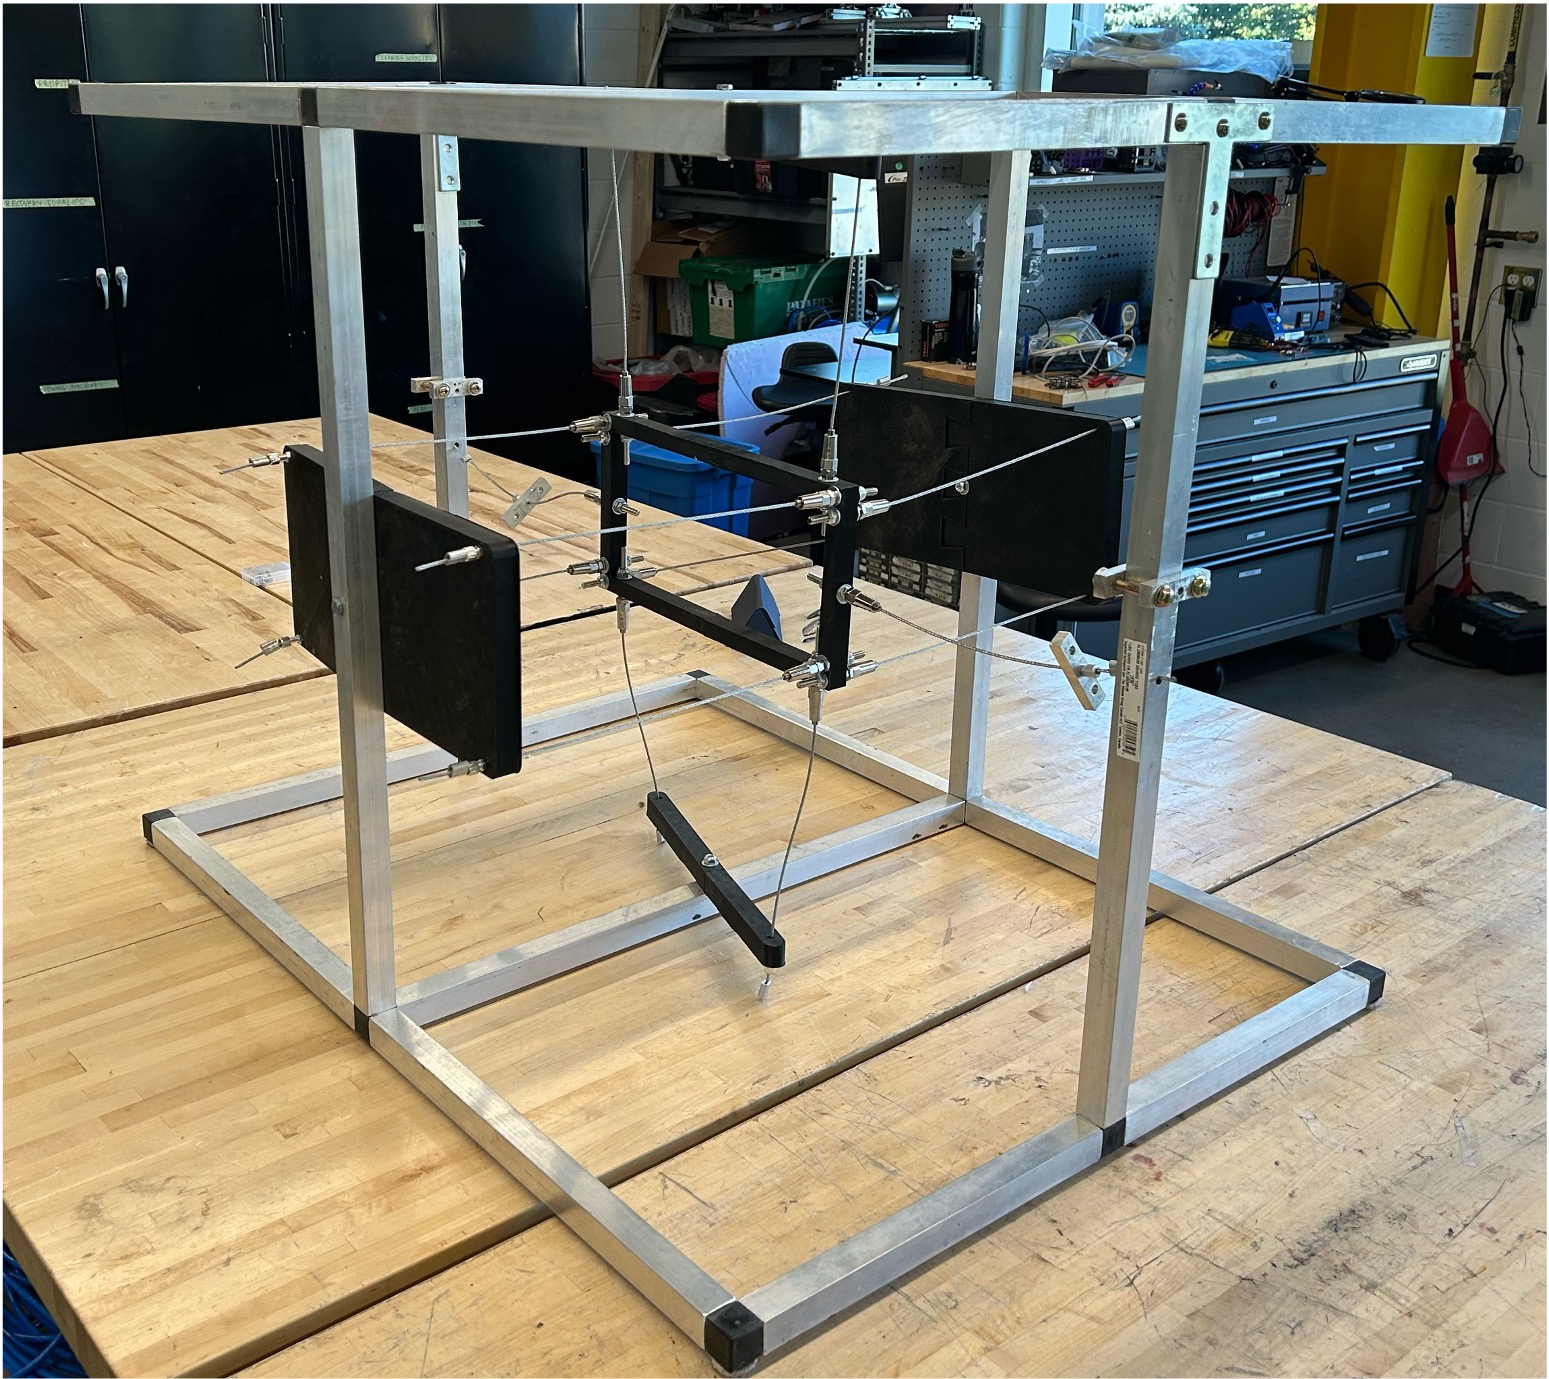
\includegraphics[height=6.5cm]{figures/State of ATP Sep 2025.jpg}
  \caption{State of the ATP at the beginning of the Fall Semester.}
  \label{fig:State_Of_ATP_Sep}
\end{figure}

Looking at Figure \ref{fig:State_Of_ATP_Sep}, we see the aluminum outer frame, 3D printed inner frame and crossbars, as well as the steel cables connecting some of the components together. During my inspections of the ATP I noticed many of the 3D printed components were prototype components and were printed in multiple pieces and glued together afterwards, creating large variations in accuracy and built quality. Additionally, I observed the barrel adjusters did not offer much adjustment for the tensioning of the steel cables, being able to tension these cables would be necessary once the time came to integrate the load cells into the ATP. Based off the recommendations of the previous year's team and my own observation I decided a re-design of the inner frame and attachment mechanism was in order.

I began by creating a CAD model of the outer frame based off the dimensions of the assembled ATP. With the outer frame accurately modelled, I could turn my attention to taking stock of the components we had on hand. I partially disassembled the ATP by removing all 3D printed components, steel cables, and couplings from the ATP. I recorded the part numbers of the couplings and measured the distances of the steel cables for later reference during the design process. Once this was complete, I was left with a bare outer frame.

\subsection{Re-Designing the Inner Frame and Couplings}

My next step was to re-design the inner frame as well as the coupling mechanism. Over the course of several weeks of iteration and design reviews with professor Garcias, I came up with a redesign of both the inner frame and coupling mechanism. 

\begin{figure}[htb]
  \centering
  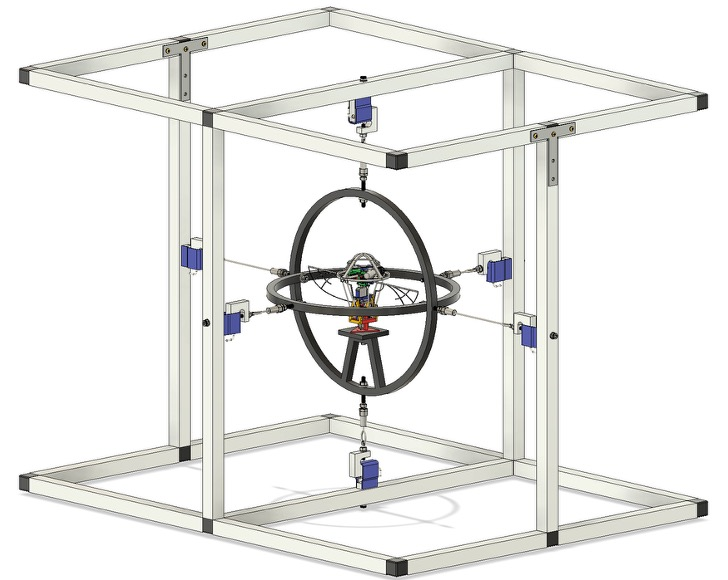
\includegraphics[height=6.5cm]{figures/Completed ATP Design.jpg}
  \caption{CAD Model of the current ATP Design.}
  \label{fig:Current_ATP_Design}
\end{figure}

The inner frame consists of two concentric 3D printed rings in addition to a 3D printed adapter plate to which the flapper can be mounted, the updated inner frame design can be seen in Figure \ref{fig:Current_ATP_Design}. As for the coupling mechanism, one side utilizes the existing stud couplers from the previous design to bolt through the inner frame. To attach the other end to the load cells, M6 stud anchors were used in conjunction with an M6 washer and nut, the steel cable could then be thread through the eyelet of the stud anchor and crimped back on itself. See Figures \ref{fig:Coupling_Mechanism} and \ref{fig:Coupling_Mechanism_Cross_Section} for a close-up view of the attachment mechanism. This attachment mechanism allowed for a large range of adjustment during the assembly process to control the tensions within the steel cables with a high degree of accuracy.

\begin{figure}
\centering
\begin{subfigure}{.5\textwidth}
  \centering
  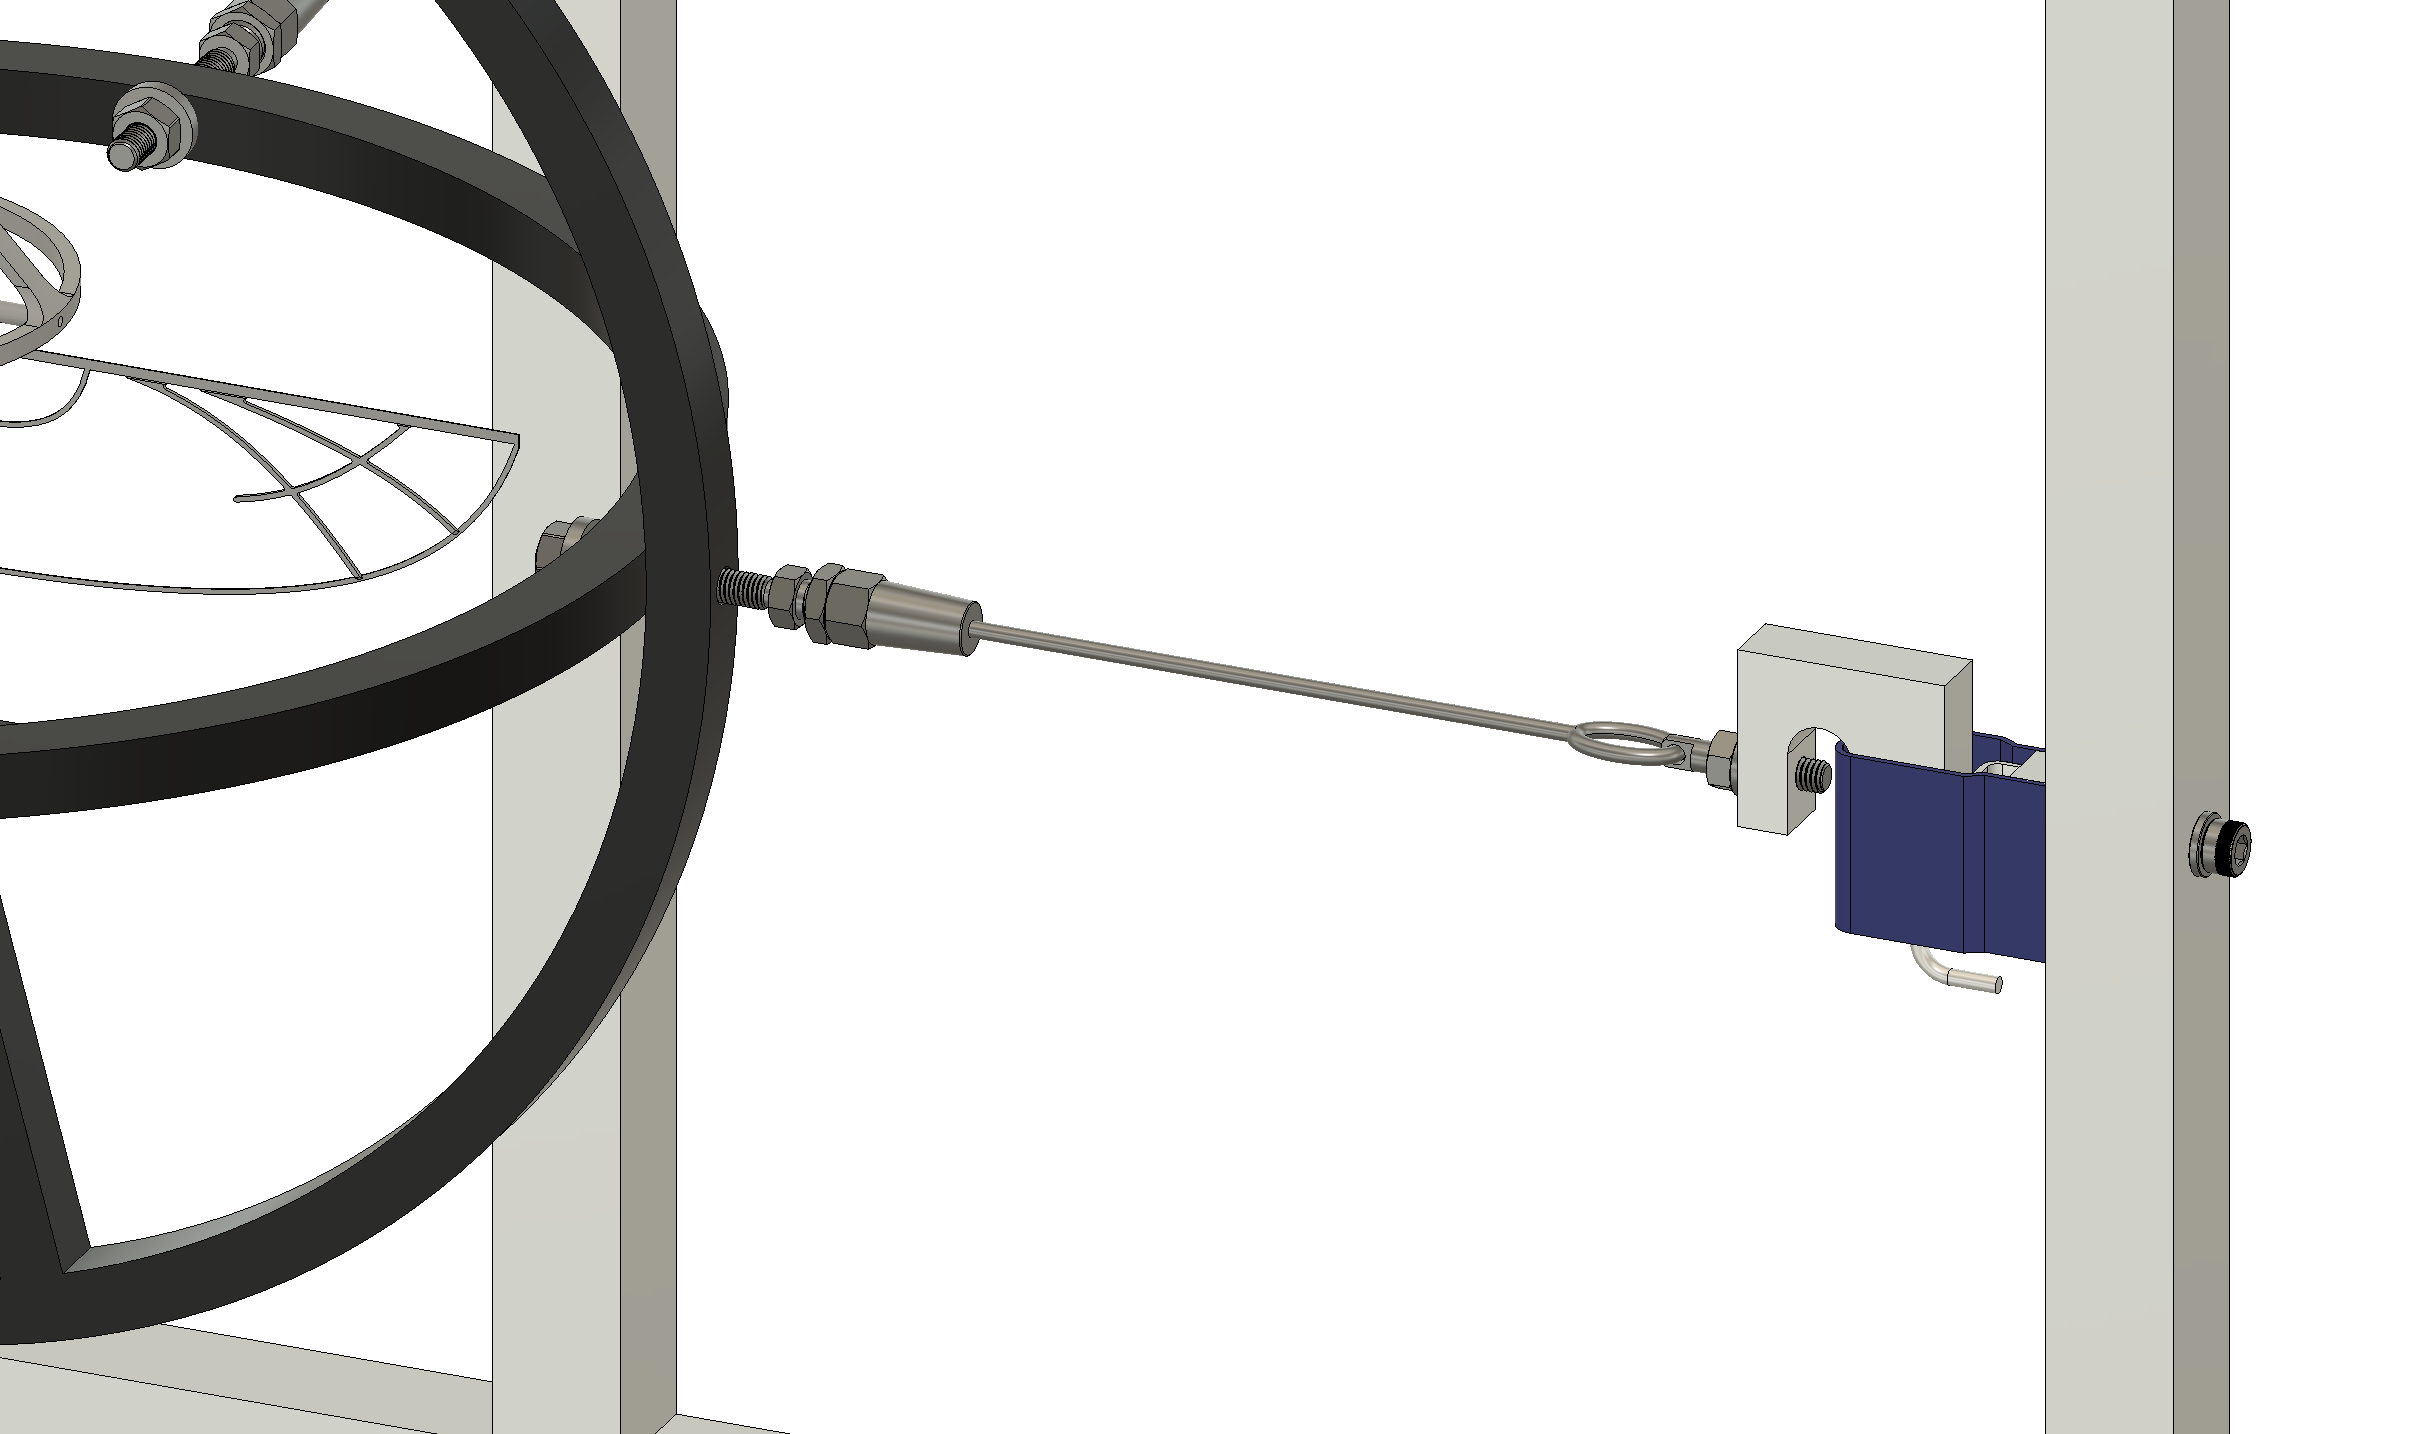
\includegraphics[height=4.5cm]{figures/Coupling Close Up.png}
  \caption{Close-Up of the Coupling Mechanism.}
  \label{fig:Coupling_Mechanism}
\end{subfigure}%
\begin{subfigure}{.5\textwidth}
  \centering
  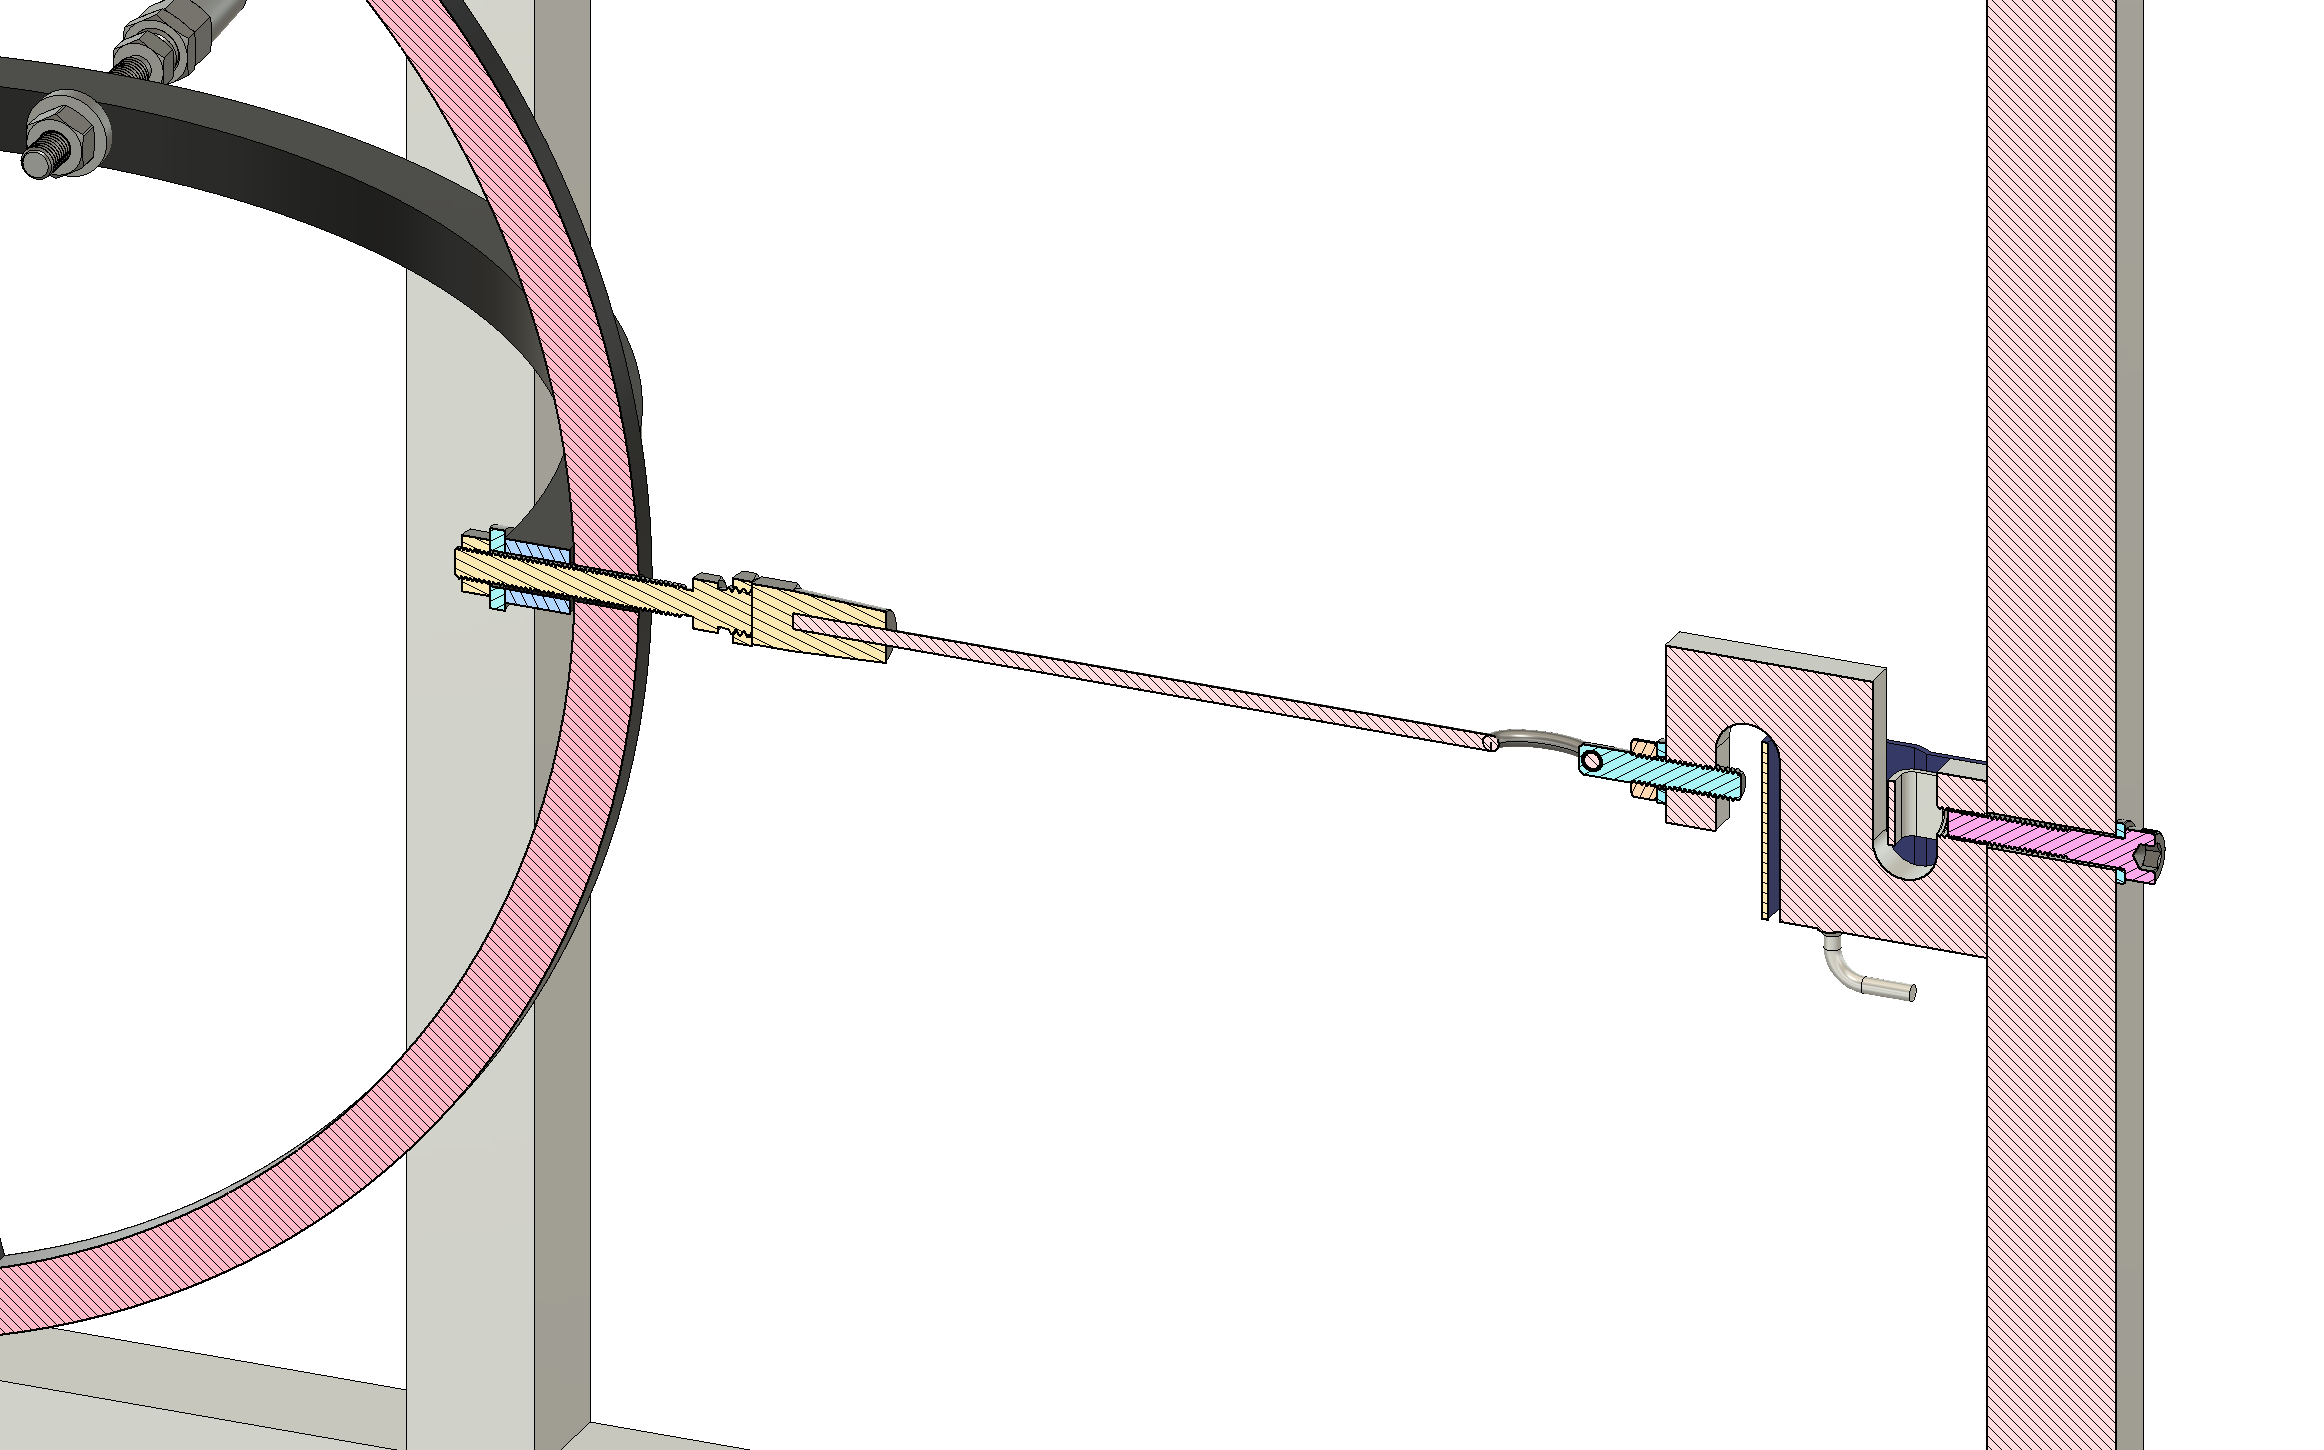
\includegraphics[height=4.5cm]{figures/Coupling Close Up Cross Section.png}
  \caption{\label{fig:right_robot} Cross Section of the Coupling Mechanism.}
  \label{fig:Coupling_Mechanism_Cross_Section}
\end{subfigure}
\caption{Detailed Views of the Coupling Mechanism.}
\label{fig:test}
\end{figure}

\subsection{Assembly and Testing}
With the design complete, it was now time to manufacture, assemble, and begin testing. The manufacturing was minimal and fast by design, only three components required manufacturing; the two 3D printed inner rings and the 3D printed adapter plate. In the meantime, the required components could be ordered from McMaster Carr. The required components consisted of mainly fasteners with the exception of the M6 stud anchors, M6 standoffs (To be used in place of the load cells during storage and assembly.), and steel cable crimp connectors.

With all components on hand the ATP could then be assembled. Assembly consisted of installing the M6 standoffs in place of the load cells, followed by measuring, cutting, and crimping the steel cables to length with the stud anchors in place. Lastly, the stud couplers could be bolted through the 3D printed inner frame rings. See Figure \ref{fig:Assembled_ATP} for an image of the assembled ATP.

\begin{figure}[htb]
  \centering
  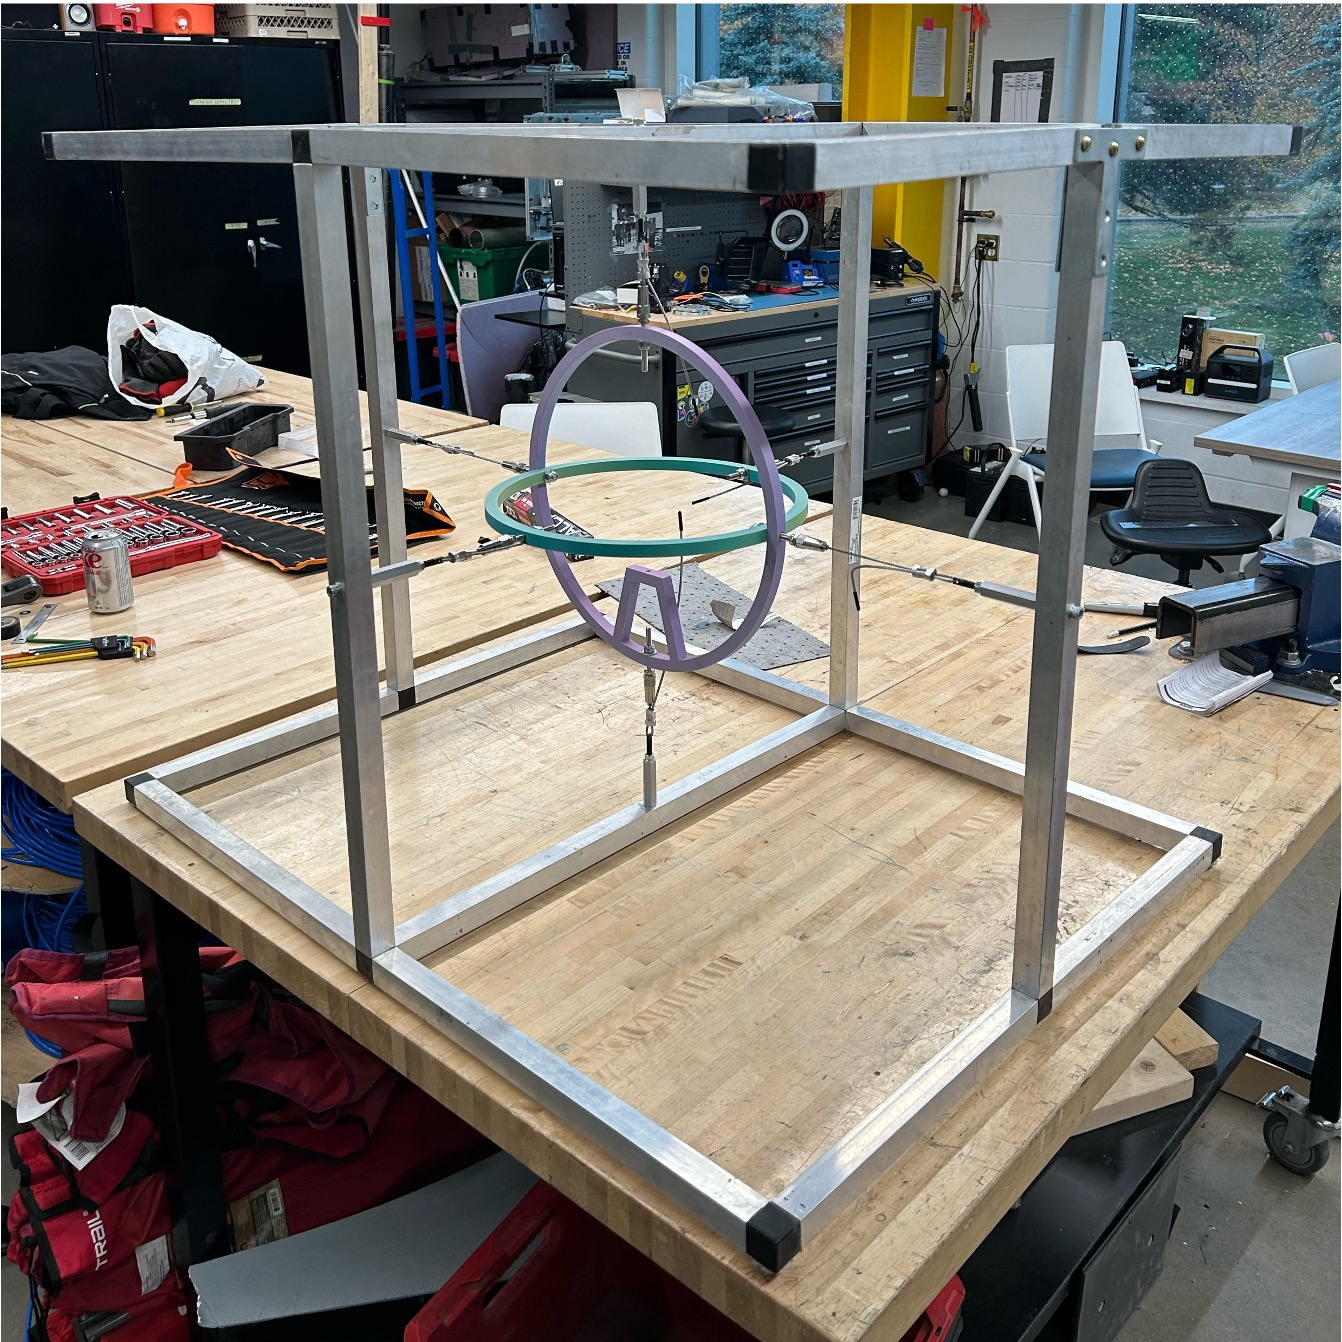
\includegraphics[height=6.5cm]{figures/Assembled ATP.jpg}
  \caption{Assembled ATP.}
  \label{fig:Assembled_ATP}
\end{figure}

With assembly complete, testing could begin. Testing is a joint effort with Kevin Fair as his role is Sensor Integration and Data Acquisition for the ATP. By this point in the semester, Kevin had gotten a single load cell functional with a laptop and LabVIEW to read the output voltage. We tested the load cell in both the horizontal and vertical orientations as well as various tensions for the steel cables. Our testing consisted of placing a series of decreasing masses onto the adapter plate and checking the output voltage of the load cell to determine the smallest detectable mass. During out initial tests, the smallest mass we detected was 200 grams. At a target flapper weight of 40 grams, this result was displeasing. Since this design utilizes steel cables, which work under tension, to achieve the desired rigidity these steel cables must be pre-tensioned. Our testing found that as this pre-tension force (And therefore the rigidity of the steel cables.) is increased, the resolution of our load cell decreased and vice-versa. Kevin talks in depth about this within section \ref{chap:Kevin_Fair} of this report. Kevin has since been able to mitigate this issue via voltage subtraction and other means discussed within his section.

With the results from our testing, my next step was to attempt to reduce the static mass of the design. With a lower static mass, the tensile forces required to support the design would be lower and therefore the resolution of the load cells could be increased.  I focused my efforts on the steel cables and couplings as these components were the heaviest. I sketched a 3D printed coupler which utilizes a bore and a tapered thread to clamp existing carbon fiber cable (Leftover from the previous year.) this coupler then connects to the thread of the load cell. This concluded my work for the fall semester.

\subsection{Plan for Winter Semester}
Moving into the winter semester, my overall goal is to get the ATP functional and able to collect data. This will primarily consist of testing and prototyping with Kevin throughout the semester.

As for the short term, I will turn my updated coupler concept into a function CAD design. I would like to design a method of adjusting the tension within the cables to help with assembly and prototyping. Once designed, manufacturing (3D printing) will occur, followed by assembly and testing. Testing will be similar to the testing process preformed previously, the load cell will be tested in a variety of orientations and analyzed using a variety of masses. Once we are satisfied with the testing results for a single load, the integration of the remaining five load cells will follow. Once all load cells our preforming as expected, data logging can begin.

\clearpage
\section{ATP Data Acquisition}
\label{chap:Kevin_Fair}
\textbf{Student:} Kevin Fair
\subsection{Background}
The previous capstone year left the data acquisition of the ATP as a proposed schematic. With hardware delivery delays, the testing performed in the previous year was limited to simulations of the system. Figure \ref{fig:LoadStringSchem} outlines this schematic as a block diagram and depicts how the suggested components are to be constructed. The three main components that the "load string" consists of are the SM S-type load cells, the AD8556 amplifiers, and the NI USB-6002 DAQ.

Going into the start of the 2025 year, the suggestion from the previous year's ATP data acquisition member was to test the hardware on the test platform. As such, the goal I outlined for this first semester was to fully commission the ATP test stand using the hardware that was proposed. My plan was to first statically load the test platform with known weights and record the measured results, then use a dynamic mechanism to reconstruct the flapping of the flyer and measure the dynamic response of the ATP.

\subsection{Method Of Analysis}
The nature of this project requires a micro aerial vehicle to fly which means the forces that it will be generating will also be micro. As such, the finest resolution that the load cells could report needed to be determined. To do this, I used a unit weight of 50 grams, as it should be close to the lift force the MFWF will generate during flight, to load and unload the load cell. This gives a method of analysis that is secluded from external factors and represents the theoretical finest resolution. In terms of quantifying the resolution, I decided to use the limit of detection (LOD) method to provide a constant way to prove the resolution for each test that was conducted.

The LOD method, represented in equation \ref{LOD}, gives a gram force resolution based on the amount of noise that is present in the signal and the deviation caused by the applied load \cite{LimitOfDetection}. This method can be applied to the measured data that has been recorded during this semester and gives a concrete way to determine the resolution of a signal. The parameter is expressed as:

\begin{equation}
\label{LOD}
    LOD = \frac{3\cdot V_{rms}}{S}
\end{equation}

where $V_{rms}$ is the root-mean-squared voltage of the noise and $S$ is the sensitivity of the the applied load in V/gram. Table \ref{tab:ATPTestResultsSummary} outlines the results of all testing carried out this semester and LOD is probably the most representative parameter that we care about.

\subsection{Preliminary System}
When the amplifiers arrived this semester, I was able to construct the load string as depicted by the schematic in Figure \ref{fig:LoadStringSchem}. 
\begin{figure}[htb]
    \centering
    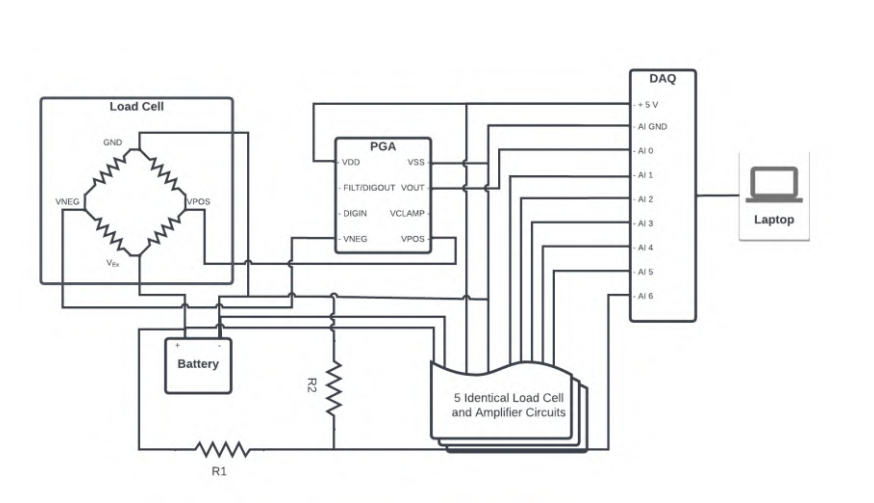
\includegraphics[height=4.5cm]{figures/PrelimSchematic.png}
    \caption{2023 Load string schematic \cite{MFWF_FinalReport2023}}
    \label{fig:LoadStringSchem}
\end{figure}
I constructed the system with one load cell that sends its signal to the input of the AD8556 amplifier, and connected the amplifier output to the borrowed NI USB-6008 DAQ as we did not have the ordered DAQ yet. My first challenge of the semester was just with this initial connection of components. The load cell is essentially just a resistor bridge; the output voltage is half the supply voltage. In this preliminary load string, the suggested voltage to power the load cell was 10 volts, but half of that (5 V) is too close to the amplifiers supply and resulted in no amplified signal. Because of this, I needed to use 5 V to the load cell, which has implications I will discuss in section 2.2.4.
\subsubsection{Unit Test}
\indent With this reduced voltage, I performed a unit test on this preliminary load string setup with gains of 70, 400, 800, and 1280 (maximum for the amplifier used), but only obtained measurable results for the 1280 gain, seen in Figure \ref{fig:Prelim1280}. The LOD (resolution) of this signal is about 30 grams. Assuming that while the lift forces of the flyer will be around the 40 gram mark, this resolution is fine enough to reliably resolve that.
\begin{figure}[htb]
    \centering
    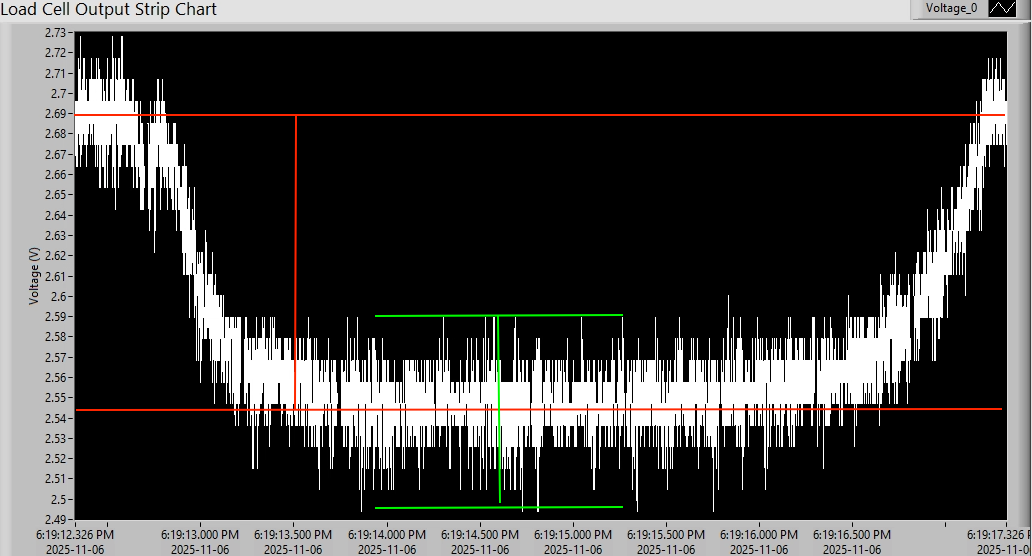
\includegraphics[height=4.5cm]{figures/Prelim1280.png}
    \caption{Preliminary load string unit test results with 1280 gain}
    \label{fig:Prelim1280}
\end{figure}
However, the purpose of the ATP is to also be able to measure any transverse loading produced by the flyer. These forces could be as low as 5 grams and with this setup, that small force would just be lost to noise. A new load string setup was required.
\subsubsection{ATP Test}
With Stan's redesign of the inner frame completed, we tested the load cells on the ATP with static loads in place for the MFWF. Unfortunately, with the tension required to fasten the load cells to the inner frame, the voltage to the DAQ exceeded its limit of +10 volts \cite{NI_USB6008_Specs}. Recall that the load cell and amplifier output a voltage proportional to the gain and applied load. To account for this, the gain was reduced in the amplifier and resulted in a minimum resolution of 200 grams. Unfortunately, this setup wouldn't be able to measure anything the flyer could produce. The load string design needed to be re-visited.
\subsection{Improved Amplifier}
One of the limitations in the preliminary load string was the amplifier. It only supported gains up to 1280 and was limited to an input of 5 volts. Amplifiers can only function if the input signal is less than its supply and recall the load cells output is half the input, meaning this amplifier restricts the load cell to 5 V. The scale of the voltage that is produced by the load cell is directly proportional to it's supply power. That is, at 5 volts, it can produce about 16 mV at its maximum load of 50 newtons (5000 grams). A 10 volt supply doubles this, such that 50 newtons is about 32 mV. What this means is that a higher supply voltage allows a larger range to represent the forces, essentially providing a higher resolution with the same gain.
\subsubsection{Unit Test}
I ordered the AD8421 which has a 32 V maximum supply (well above 5 V), and could apply gain up to 2000 \cite{Analog_AD8421_Datasheet}. Using this, I was able to push the load cell supply to 10 V and performed another unit test. Figure \ref{fig:NewAmpUnitTest} shows the results of the test as the unit load is unloaded. The figure is comparatively more discrete than Figure \ref{fig:Prelim1280}.
\begin{figure}[htb]
\centering
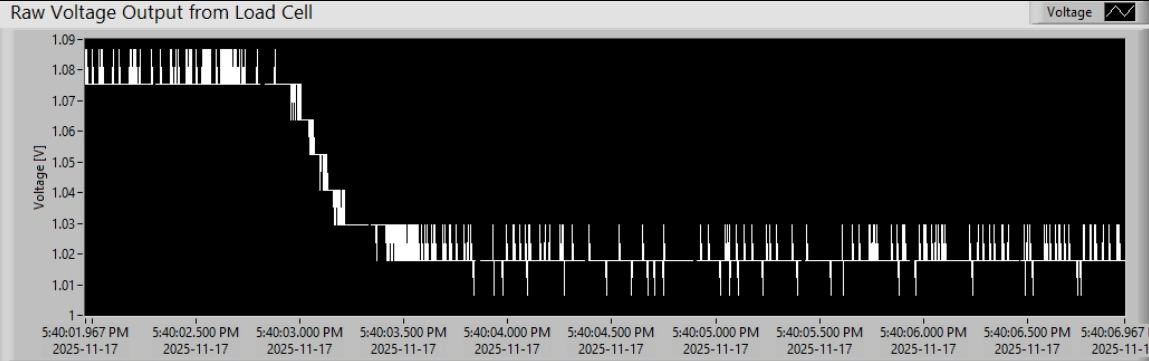
\includegraphics[height=4.5cm]{figures/NewAmpUnitTest.png}
\caption{New amplifier unit test with 2000 gain}
\label{fig:NewAmpUnitTest}
\end{figure}
This was actually due to the limits of the USB-6008 DAQ that was borrowed. It has a 12-bit analog to digital converter (ADC) \cite{NI_USB6008_Specs} which means that the smallest discrete "steps" it can turn an analog signal into is 0.005 V. of 0.01 V. Regardless of this, the test resulted in an LOD of 19 grams; better than the previous setup by about 11 grams, but still not small enough for the ideal of 5 grams.
\subsubsection{ATP Test}
The issue of tension was still present when wanting to test this load string on the ATP. It reached a point where it was thought a new ATP design would be needed to remove the tension in the load cells for a proper reading to be achieved. 
\subsection{Subtracting the Tension}
After discussing the tension problem in one of the weekly presentations, Professor Hashim provided a very insightful suggestion of subtracting the voltage that the tension produces with another known (static) voltage. This allowed the small force produced by the MFWF to be isolated and gained independently of the tension force.

I achieved subtraction by utilizing another AD8421 amplifier. The amplifier is made from op-amp stages that amplify its inputs and subtracts the signals. The first amplifier would take the load cell output and multiply it by some gain such that the output was 10 V plus the small load of the MFWF. I would then use that as an input to the next amplifier and the other input was a clean 10 V, resulting in just the small loads of the flapper as a relatively large voltage. Figure \ref{fig:BBDifference} shows just how many extra components that went in to achieve this subtraction, although most are just for power distribution.
\begin{figure}[htb]
\centering
\begin{subfigure}[t]{.5\textwidth}
  \centering
  \includegraphics[height=4.5cm]{figures/DAQ_BB_Init1.png}
  \caption{Preliminary setup}
  \label{fig:PrelimBB}
\end{subfigure}
\begin{subfigure}[t]{.5\textwidth}
  \centering
  \includegraphics[height=4.5cm]{figures/DAQ_BB_Final1.png}
  \caption{Subtraction setup}
  \label{fig:FinalBB}
\end{subfigure}
\caption{Breadboard setups for (a) preliminary and (b) subtraction load string designs}
\label{fig:BBDifference}
\end{figure}

\subsubsection{Unit Test}
While the new design was modified for testing on the ATP, the USB-6002 DAQ had arrived during the same time period. Instead of a 12-bit ADC, it used a 16-bit ADC \cite{NI_USB6002_Specs}, which allowed finer step sizes to be measured on a signal. To verify this, I performed another unit test with the same setup as in section 2.2.4, but with the new DAQ. Figure \ref{fig:NewDAQUnitTest} shows the measurement of this unit test and compared to Figure \ref{fig:NewAmpUnitTest}, 
\begin{figure}[htb]
    \centering
    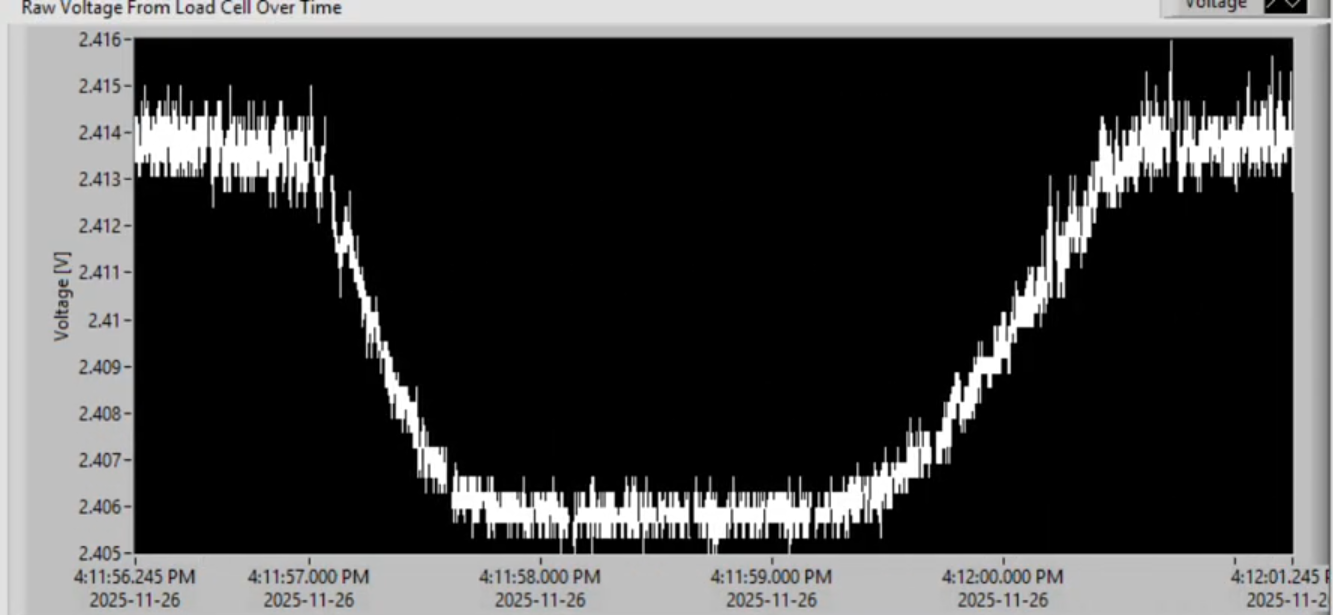
\includegraphics[height=4.5cm]{figures/NewDAQUnitTest.png}
    \caption{USB-6002 DAQ unit test load and unload}
    \label{fig:NewDAQUnitTest}
\end{figure}
it is visually quite an improvement. In fact, the LOD of this test was calculated to be 6.6 grams. Although this resolution is very close to the goal of 5 grams, the load cells themselves have an inaccuracy of 2.5 grams (0.025 N) \cite{Interface_SM_SType}. This means that with the current load cells, we would never be able to measure any force at the scale of the MFWF with 100\% accuracy. Even the thrust could be reported as 50 grams when it is actually 47.5 grams.
\subsubsection{ATP Test}
The ultimate goal of this semester was to commission of the ATP using the hardware we had. Since section 2.2.3 proved that the hardware we had was not adequate, I used the subtraction load string to perform the basis of the commissioning. I fastened a load cell to the top of the ATP and placed different weights on the inner frame to achieve a range of results. The subtraction load string was able to remove the tension while recording the signal. The result was a significant improved measurement of the applied loads. Figures \ref{fig:100gATPLoad} to \ref{fig:10gATPLoad} show the loading or unloading of four different applied loads.
\begin{figure}[htbp]
    \centering
    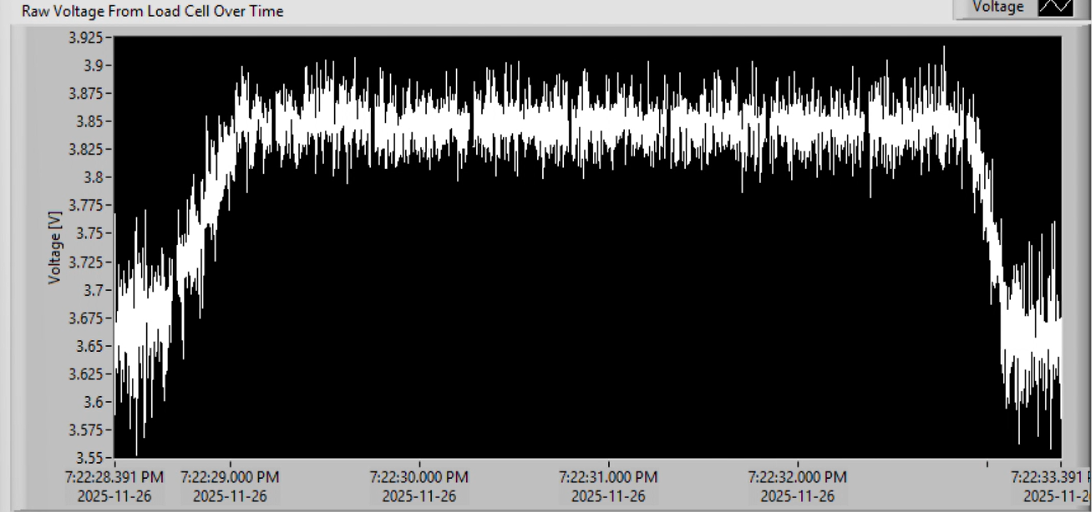
\includegraphics[height=4.5cm]{figures/DoubleAmp_100.png}
    \caption{100-gram ATP test load and unload}
    \label{fig:100gATPLoad}
\end{figure}
\begin{figure}[htbp]
    \centering
    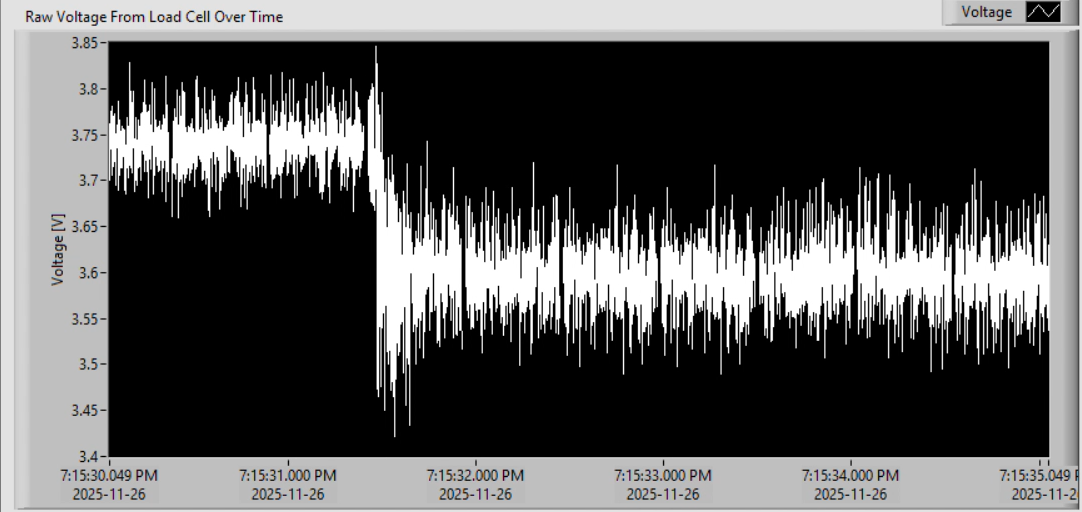
\includegraphics[height=4.5cm]{figures/50g_doubleAmp.png}
    \caption{50-gram ATP test unload}
    \label{fig:50gATPLoad}
\end{figure}
\begin{figure}[htbp]
    \centering
    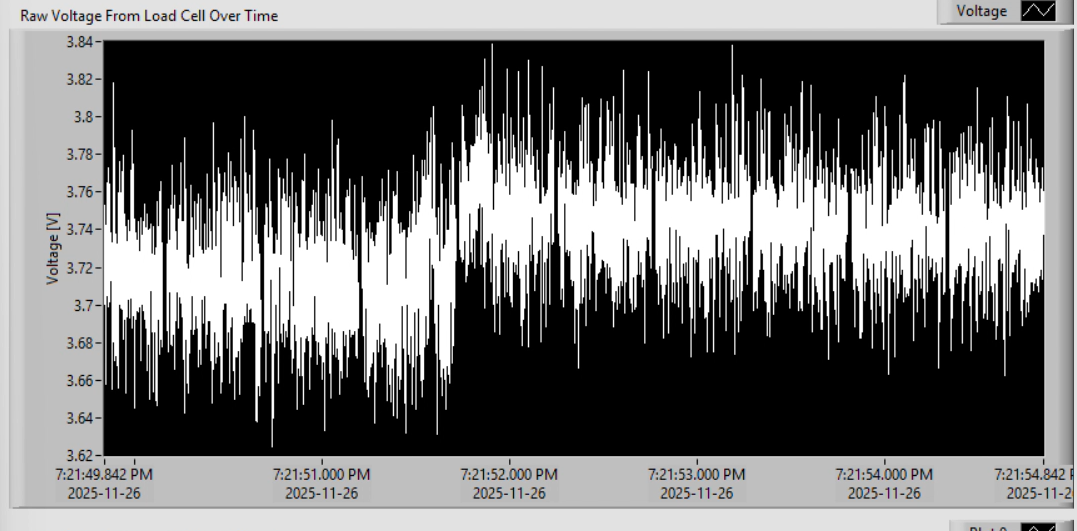
\includegraphics[height=4.5cm]{figures/DoubleAmp_20.png}
    \caption{20-gram ATP test load}
    \label{fig:20gATPLoad}
\end{figure}
\begin{figure}[htbp]
    \centering
    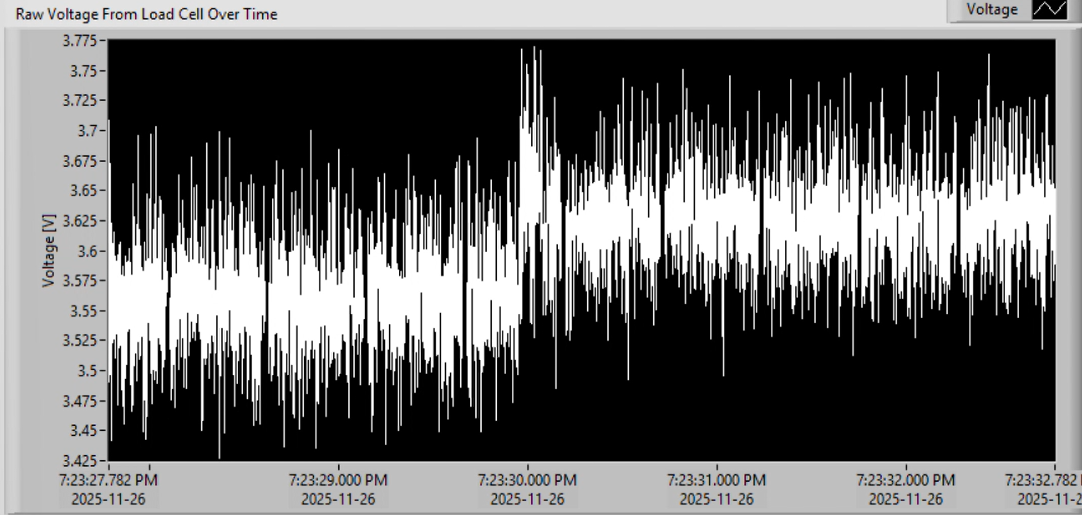
\includegraphics[height=4.5cm]{figures/DoubleAmp_10.png}
    \caption{10-gram ATP test load}
    \label{fig:10gATPLoad}
\end{figure}

Table \ref{tab:ATPTestResultsSummary} shows that the best LOD of the ATP comissioning was 26.6 grams, which represents the 100-gram loading condition. This result is still not as ideal as I'd prefer, but compared to 200 grams, its a large improvement. I do believe that with some tweaking of the load string and some filtering of the signal, it can be viable. An important consideration, however, is the dynamic load of the flapper. With loading and unloading at about 40 Hz frequency, I'm not confident that same resolution can be achieved.

\subsection{Testing Results Summary}
Table \ref{tab:ATPTestResultsSummary} summarizes all the testing that was performed this semester with the different load string designs.
\begin{table} [htbp]
    \centering
    \begin{tabular}{||c|c|c|c||}
        \hline
        Test & $V_{rms}$ Noise $[mV]$ & $S$ [$\frac{mV}{g}$] & $LOD$ [g] \\
        \hline\hline
        Preliminary Unit & 28.3 & 2.8 & 30.3 \\
        \hline
        New Amp. Unit & 7.07 & 1.1 & 19.3 \\
        \hline
        New DAQ Unit & 0.354 & 0.16 & 6.64 \\
        \hline
        ATP Calibration (Best) & 35.4 & 4 & 26.6 \\
        \hline
    \end{tabular}
    \caption{Fall semester ATP test results summary}
    \label{tab:ATPTestResultsSummary}
\end{table}

\subsection{Plan for Winter Semester}
In terms of the signal resolution for a unit load, the load string is capable of determining a load close to the desired 5-gram resolution. However, the load cells inherent accuracy of 2.5 grams limits the fine readings that can be achieved. In terms of ATP comissioning, the subtraction load string is clearly beneficial to remove the tension effects of the current design, but the signals at smaller loads are still quite noisy. The winter semester should have me focusing on improving this signal quality by using some sort of filtering technique.

However, the filtering will have an effect on the dynamic response of the system. While the fine measurements (sub 20 grams) are harder to measure on the ATP, I believe the dynamics of the flyer will have a large impact on the resolution of this signal, and a point should be made to verify a dynamic resolution of even 50 grams if the team is to use this ATP design. The first priority of the winter semester should be to test the ATP with a dynamic load that simulates the flapping of the MFWF. With the results of this test, and some tuning of the subtraction load string, I indent to have a reasonable understanding of how the ATP will perform with the MFWF mounted. Given that professor Hashim has been influential to this side of the ATP team, I will be using him as a resource to gain more knowledge of how the fine resolution of a dynamic flyer can be achieved. Ultimately, my goal before the winter semester ends is to have an exhausted testing report of this ATP design to prove its viability for the MFWF team to use during their flight tests. 

\newpage
\section{LSTM Neural Network Development}
\label{chap:Wade_Schnurr}
\textbf{Student:} Wade Schnurr
\subsection{Background}
There is no previous progress to refer to, as the machine learning roles of the Aerodynamic Test Platform and Wings (ATPW) subgroup are newly defined responsibilities.

\subsection{Introduction}
The overall goal for the neural network is to develop a non-linear black-box aerodynamic model using a machine learning model to predict three-dimensional aerodynamic forces to validate and compare with the 
experimental data obtained from the Aerodynamic Test Platform (ATP). Eventually, for comparison, two different machine learning approaches, such as neural networks, will be used to model the non-linear aerodynamics of flapping wings. The team has currently collected aerodynamic data on NACA airfoils to synthesize and validate aerodynamic models as a preliminary exercise.

\subsection{Analysis of Problem}
Before steps could be taken towards developing a model, an understanding of machine learning (ML) to a certain level had to be established. This was done through online resources, for example, online lectures presented by Andrew Ng at Stanford \cite{NgDeepLearningPlaylist2025}, YouTube video series such as Deep Learning With Tensorflow 2.0, Keras and Python by codebasics \cite{codebasicsDeepLearning2025}, podcasts such as the Machine Learning Guide by OCDevel \cite{OCDevelMLGSpotify2025}, discussions with the assigned Lead Engineer Professor Hashim A. Hashim Mohamed, and more. For future groups, Andrew Ng's Coursera course was also often recommended.

\subsubsection{Dataset Preparation}
Before a machine model could be selected and created, a dataset needed to be selected. NACA airfoil data were chosen for the preliminary exercise. The NACA airfoil data were selected because there appeared to be some rough correlation and potential overlap between the categories of data presented for the NACA airfoils and the potential data to be extracted from the Micro Flapping-Wing Flyer (MFWF) and ATP. Joukowsky and NACA 4, 5, 6, and 7 digit airfoil data were extracted from airfoiltools.com \cite{AirfoilToolsNACA4Digit2025}. Each airfoil on airfoiltools.com was divided into seven files, each containing data for one of the seven Reynolds-number intervals from 50,000 to 5,000,000. Initially, to develop the ML model, a small sample of airfoil data was downloaded as a Microsoft Excel file and combined to enable faster training and iteration. Over time, as the ML model was developed, Aidan Sheridan compiled a large Excel dataset containing all available airfoils and associated information, adding two new columns: one for the NACA Airfoil ID and another for the Reynolds Number. A few refinements were applied to the large dataset to make it easier for the ML model to read, and the model was then trained on it. There are six categories of information that were available with each NACA airfoil: angle of attack (\( \alpha \)), transition point on upper and lower surface (Top\_Xtr and Bot\_Xtr), Reynolds Number (Re), lift coefficient (Cl), drag coefficient (Cd), pitching moment (Cm), and profile drag coefficient (Cdp).

\subsubsection{Machine Learning Model Development}
The machine learning (ML) model for the preliminary exercise was to predict / output four values, the lift coefficient (Cl), drag coefficient (Cd), pitching moment (Cm), and profile drag coefficient (Cdp) based on five input parameters, NACA airfoil ID, angle of attack (\( \alpha \)), transition point on upper and lower surface (Top\_Xtr and Bot\_Xtr), and Reynolds Number (Re).

The initial ML approach led to the development of a Long Short-Term Memory (LSTM), a type of Recurrent Neural Network (RNN), as recommended based on in-class feedback. An LSTM model is designed for time-series/sequential data, data that depends on previous data points, streams of data. For example, predicting the weather depends on current and previous conditions and how they have changed over time. However, the NACA airfoil data is not sequential; it does not depend on the data before or after it. Each row of data is independent and can be randomly ordered; this would not affect the prediction. The LSTM model added complexity without improving prediction accuracy. Early tests showed that the LSTM model underperformed, particularly when the NACA airfoil ID was not used as an input parameter (four inputs instead of five) compared to other models discussed later. LSTMs require 3-dimensional input (batch, time, and features). Since the NACA airfoil data was not sequenced, no time dimension, requiring the addition of a forced fake sequence that provided no meaningful context to the model, adding unnecessary complexity and slowing it down. Overall, the LSTM model had an increased training time, memory usage, and hyperparameter sensitivity.

A Multi-Layer Perceptron (MLP) model was trained as it was better suited to the NACA airfoil dataset. An MLP was chosen because the NACA airfoil data is not sequential; it is static. MLP models can take an input of a simple list of numbers and learn relationships among them. The aerodynamic coefficients being predicted depend on complex interactions among variables, and MLP models can learn these nonlinear patterns to a relatively high degree of accuracy. MLP models contain fewer layers and complications, resulting in a simpler architecture compared to the previous LSTM model.

\subsubsection{Model Evaluation and Validation}

To assess the accuracy of the trained model, two main plots are utilized. Figures~\ref{fig: LSTM 2: Pred vs True Coefficients} and~\ref{fig: MLP: Pred vs True Coefficients} depict the true coefficient as the x-coordinate and the associated models prediction as the y-coordinate. The line y=x represents where the predictions perfectly represent the true coefficient, and the farther the distance from the line, the worse the prediction is. Figures~\ref{fig: LSTM 2: Training Accuracy} and~\ref{fig:MLP: Training Accuracy} show the system's accuracy using mean squared error (MSE) loss as a function of Epoch, the number of times the model has gone through the dataset.

\begin{figure}[htbp]
    \centering
    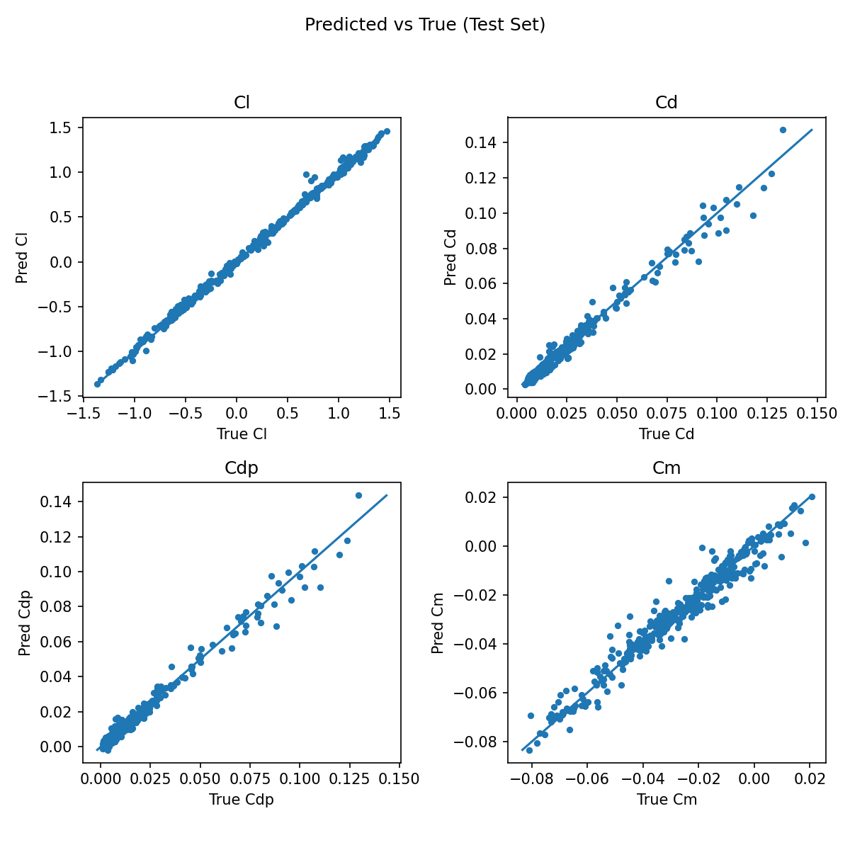
\includegraphics[width = 10 cm]{figures/Wade Schnurr Images/LSTM 2 Predicted vs True (Test Set).png}
    \caption{LSTM model version 2, predicted coefficient results compared to the actual coefficient values.}
    \label{fig: LSTM 2: Pred vs True Coefficients}
\end{figure}

\begin{figure}[htbp]
    \centering
    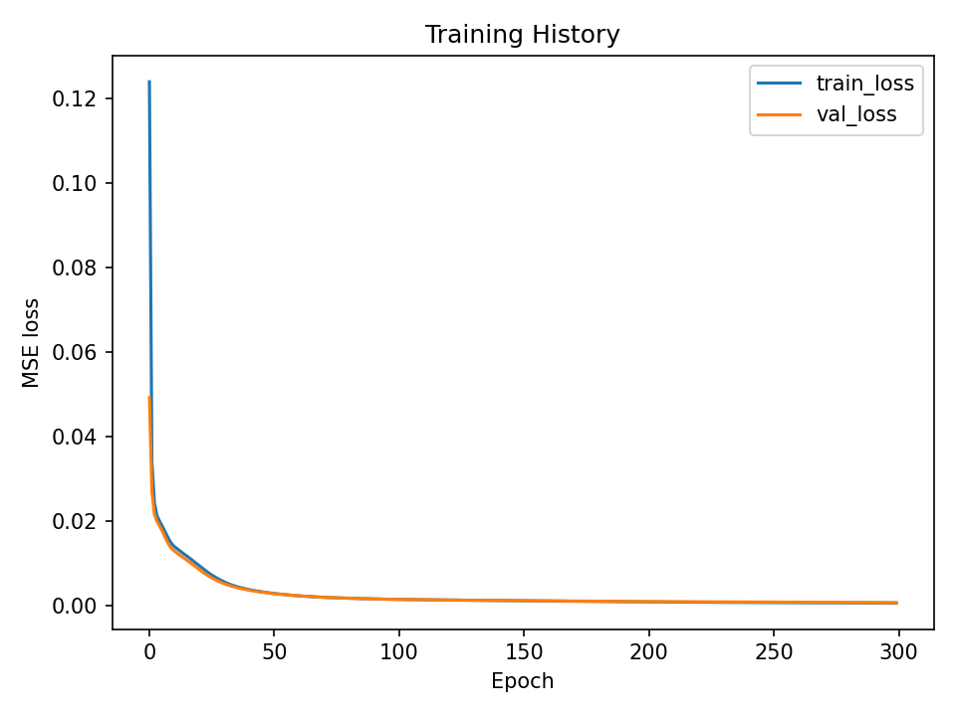
\includegraphics[width = 10 cm]{figures/Wade Schnurr Images/LSTM 2 with Arifoil Training History.png}
    \caption{LSTM model version 2, training accuracy compared to the number of times the dataset has been run through.}
    \label{fig: LSTM 2: Training Accuracy}
\end{figure}

\begin{figure}[htbp]
    \centering
    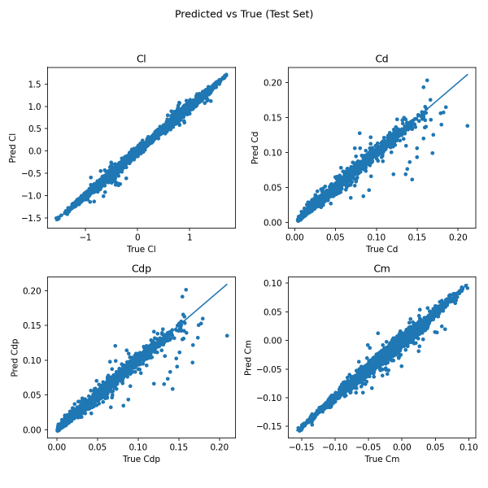
\includegraphics[width = 10 cm]{figures/Wade Schnurr Images/MLP Predicted vs True (Test Set).png}
    \caption{MLP model predicted coefficient results compared to the actual coefficient values.}
    \label{fig: MLP: Pred vs True Coefficients}
\end{figure}

\begin{figure}[htbp]
    \centering
    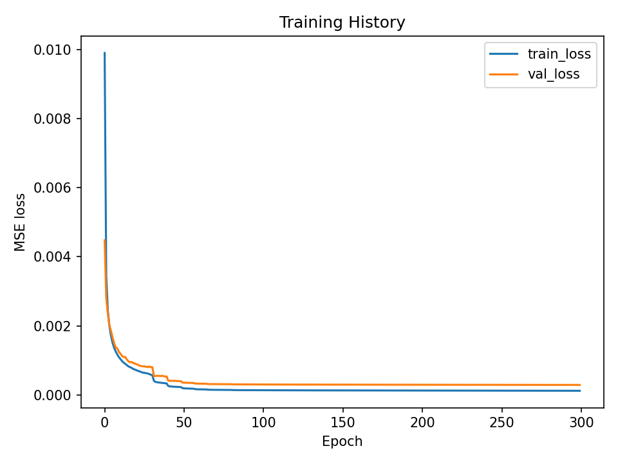
\includegraphics[width = 10 cm]{figures/Wade Schnurr Images/MLP Training History (Large NACA Airfoil Dataset).png}
    \caption{MLP model training accuracy compared to the number of times the large dataset has been run through.}
    \label{fig:MLP: Training Accuracy}
\end{figure}

\newpage
\subsection{Plan for Winter Semester}
At this time, there are two main goals for the ATPW machine learning group to continue progress into the winter semester. One: determine relevant ways to interpret and display the information generated by the current MLP model trained on NACA airfoil data. Two: consider the data that will be used as inputs and outputs from the ATP, how the X, Y, and Z forces are produced and their format. Analyze whether the current MLP model can be modified to accept the information from the ATP and produce high-accuracy results, or if it is necessary to develop a new model better suited for the type of data generated by the ATP.

\newpage
\section{MLP Neutral Network Development}
\label{chap:Aidan_Sheridan}
\textbf{Student:} Aidan Sheridan
\subsection{Background}
 
This year, a new sub-team was created to develop a non-linear black-box model to analyze and predict the aerodynamic forces on the flapping wings of the micro-flapping wing-flyer utilizing neural networks. As this was an entirely new sub-team that was created this year, the team had to start from the ground up researching different models and figuring out which would be the best fit for accurately predict the three-dimensional forces.
 
\begin{figure}[htb]
  \centering
  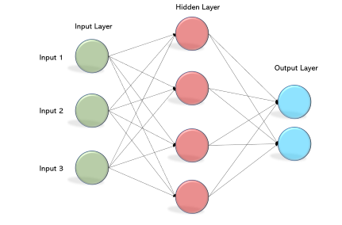
\includegraphics[height=6.5cm]{figures/MLP Network Diagram Aidan.png}
  \caption{Architecture of an MLP model.}
  \label{fig:MLP_Architecture}
\end{figure}
 
The team settled on researching two different neural network types and determining how they function, and how they could be used to predict the aerodynamic forces. I decided to focus on a Multilayer Perceptron (MLP) model, which is made up of input, output and hidden layers, where the hidden layers allow the network to handle nonlinear problems. The different layers are connected by a series of neurons that each take an input and  processes it to produce an output. Each neuron has a weight that determines importance, and these weights are summed and passed through an activation function, which introduces nonlinearity to the function.
 
\subsection{Training Data}
To build the network, I made a test network that can predict the coefficient of lift, coefficient of drag, pressure drag coefficient, and the pitching moment coefficient from the angle of attack, Reynolds number, and the top and bottom transition points of various airfoils. I used a database of NACA airfoils that I gathered from "splinecloud.com" which provided a large database of various NACA airfoils and the necessary input and output parameters for the network, and compiled them into a single excel file that contained over 66,000 individual samples of data across 619 different airfoils. This excel sheet listed out all the parameters required for the network, and was also used by Wade Schnurr for his work on the Long Short-Term Memory (LSTM) model that was occurring simultaneously with my model.
 
\begin{figure}[htbp]
  \centering
  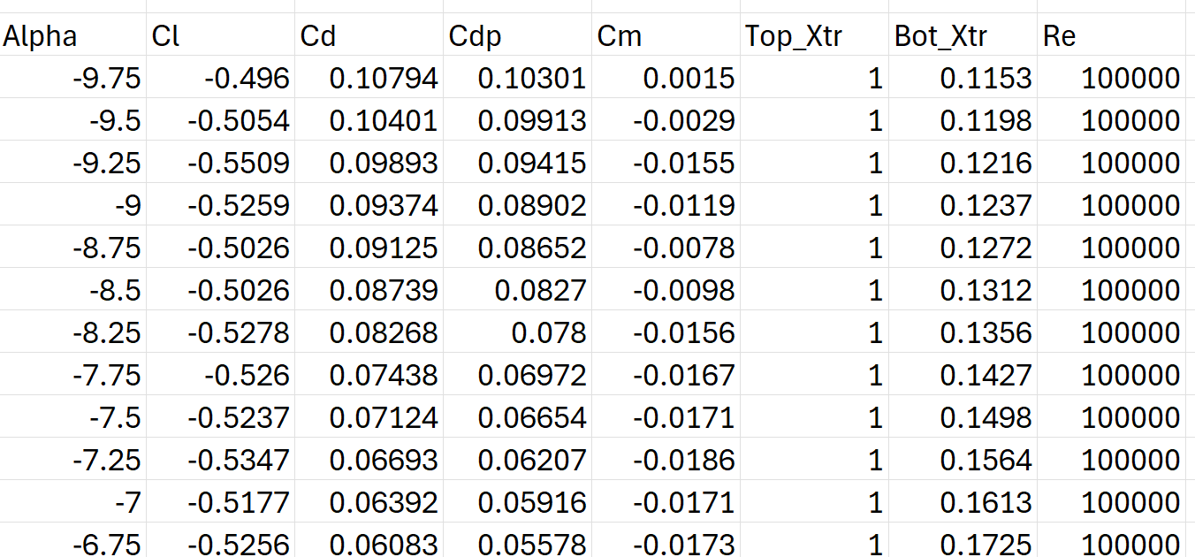
\includegraphics[height=6.5cm]{figures/Training Data Aidan.png}
  \caption{Samples of NACA Airfoil Training Data.}
  \label{fig:NACA_Airfoil_Training_Data}
\end{figure}
 
\subsection{Model and Results}
 
\begin{figure}[htbp]
  \centering
  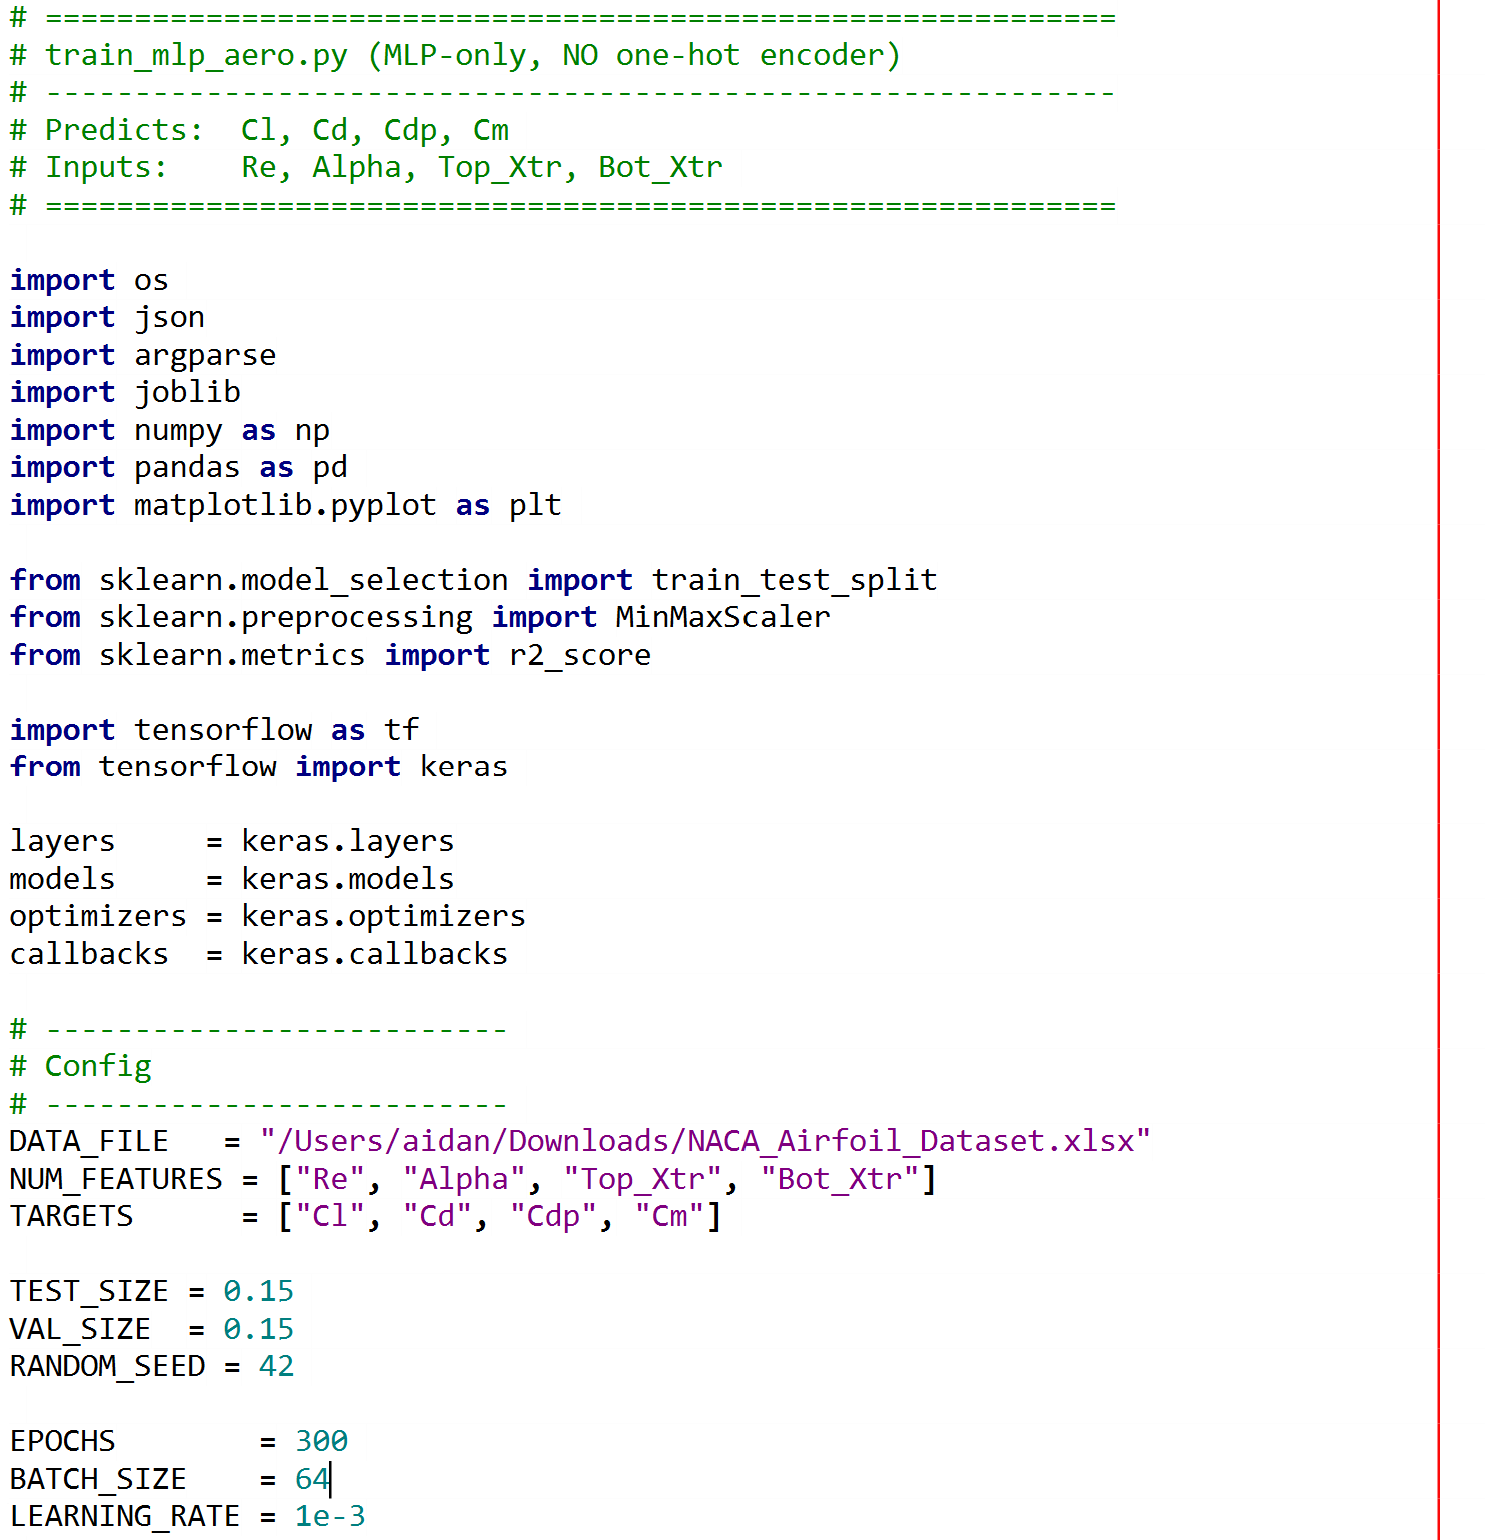
\includegraphics[height=10cm]{figures/Aidan Code Image 1.png}
  \caption{Sample of the MLP Network Code Used in Training Model.}
  \label{fig:MLP Code}
\end{figure}
 
The network that I used had three hidden layers due to the complexity of the network with 4 inputs and outputs, and included 452 neurons, which are 256, 128 and 64 in the hidden layers, and 4 for the input layer as is standard for MLP networks. The network included a Rectified Linear Unit (ReLU) activation function, which outputs 0 for negative inputs and the input itself for positive inputs, which is useful for modeling complex relationships in data. The network also has a dropout function, which randomly deactivates neurons during training in order to prevent over-fitting.
 
\begin{figure}[htb]
  \centering
  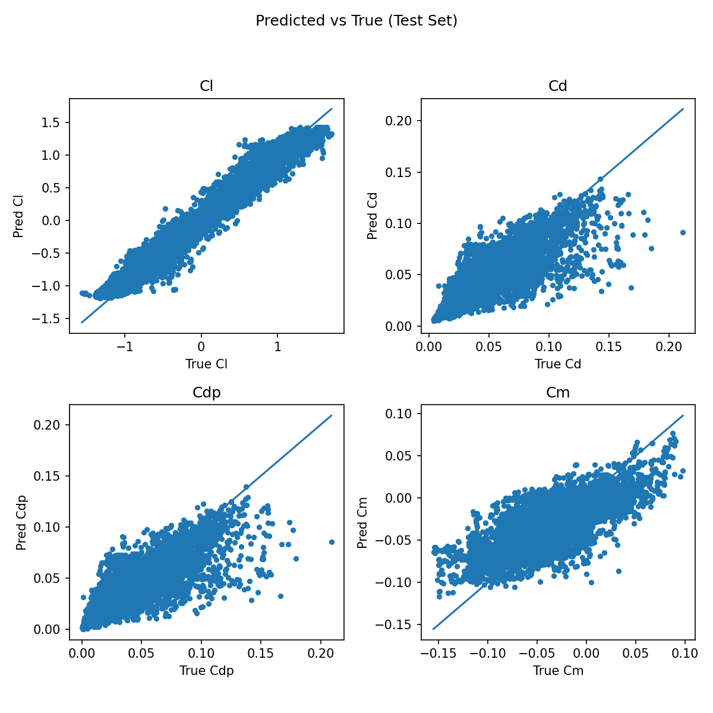
\includegraphics[height=6.5cm]{figures/Predicted vs True Aidan.png}
  \caption{Predicted vs. Real Values of Parameters.}
  \label{fig:Predicted_vs_Real}
\end{figure}
 
\begin{figure}[htbp]
  \centering
  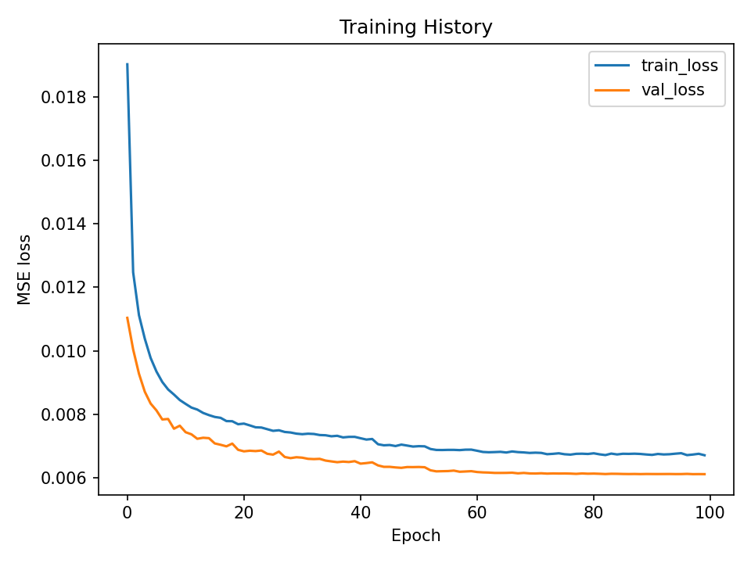
\includegraphics[height=6.0cm]{figures/Training and Validation Loss Aidan.png}
  \caption{Training and Validation Losses throughout Training}
  \label{fig:Training_and_Validation}
\end{figure}
 
\begin{table}[htbp]
    \centering
    \begin{tabular}{|c|c|}
        \hline
        Accuracy Type & Accuracy Percentage \\ \hline
        Training Accuracy & 90.4805 \\ \hline
        Validation Accuracy & 91.8836 \\ \hline
        Test Accuracy & 96.304 \\ \hline
    \end{tabular}
    \caption{Training, Validation, and Test Accuracies}
    \label{tab:four_by_two}
\end{table}
 
\newpage
The training, validation and test accuracies were found to be 0.904805, 0.918836 and 0.963504 respectively. The accuracies can be increased with more epochs and a smaller batch size, where 100 epochs were used with a batch size of 64. Overall, this is good progress for the network.
 
\subsection{Plan for Winter Semester}
Next semester, the team will focus on using the model to predict the three-dimensional aerodynamic forces acting upon the flapping wings. Once the model is accurate enough, the input parameters will have to be determined and sufficient data will have to be collected by the rest of the ATPW team in order to be able to predict these forces.

\newpage
\section{Wing Design and Manufacturing}
\label{chap:Abdulrahman_Sirajudeen-Sanni}
\textbf{Student:} Abdulrahman Sirajudeen-Sanni 
\subsection{Background}

The previous wing design team worked on developing a lightweight, manufacturable wings for the flyer and made several key contributions. In 2022, the team established an initial test framework by building a static deflection test stand capable of measuring deflection at 3 points (root, mid, and tip) along the span of the wing. This allowed for early comparison of different combinations of veins and membranes, and a database was created using the results obtained. In the static tests, the team explored a wide range of vein geometries and materials, including LW-PLA and PETG, with carbon fibre leading edge rods. The root control bar as designed by the flapping mechanism team in the same year was also incorporated in the wing.These efforts helped identify  structural issues such as excessive stiffness, excessive deformation at the trailing edge, and durability concerns. The final design was selected based on performance in the static tests and initial project requirements. 

Some work was done to characterize membrane materials such as polypropylene tape, Kapton, and RC covering film. The team observed that the membrane stiffness and vein geometry strongly influenced camber formation and overall deformation quality. Additionally, the team Identified root vein weaknesses. This revealed the need for reinforcement at the wing root to survive inertial loading at 30 Hz during stroke reversal.

Overall, a database of 12 prototype wings, documenting each design’s weight, geometry, and deformation profile was produced. Although static tests do not fully predict dynamic performance, the results helped in the selection of a wing design to compare results obtained this year to. The previous work also provided a foundation of viable materials and manufacturing processes for MFWF wings. These were used in the new prototypes developed this year. As the wing requirements remain the same this year, the insights from their work shaped this year’s focus on achieving controlled camber, improved stiffness gradients in vein geometry, and dynamic testing of new wing designs. The following are the requirements and constraints for the MFWF wing.

\begin{enumerate}
    \item The wing must be able to provide sufficient lift to the flyer.
    \item The wing must provide a means of attitude control via root actuation.
    \item To ensure the flyer is controllable, the wings must deform in a uniform and predictable manner.
    \item The wings must meet the following physical constraints
    \begin{enumerate}
        \item Each wing may have a span of up to 10 cm.
        \item Each wing can weigh up to 1.5 grams.
    \end{enumerate}
    \item The wing must be able to withstand the forces imparted on it for the duration of the flight. There are two peak loads of concern:
    \begin{enumerate}
        \item Peak inertial loads experienced during stroke reversal.
        \item Peak aerodynamic loads experienced at mid-stroke.
    \end{enumerate}
    \item The wings should be easy to manufacture and with consistent results.
\end{enumerate}

Figure \ref{fig:baselinewingmodified} shows the wing made of LW-PLA veins and Kapton tape designed by the previous teams. 

\begin{figure}[htb]
    \centering
    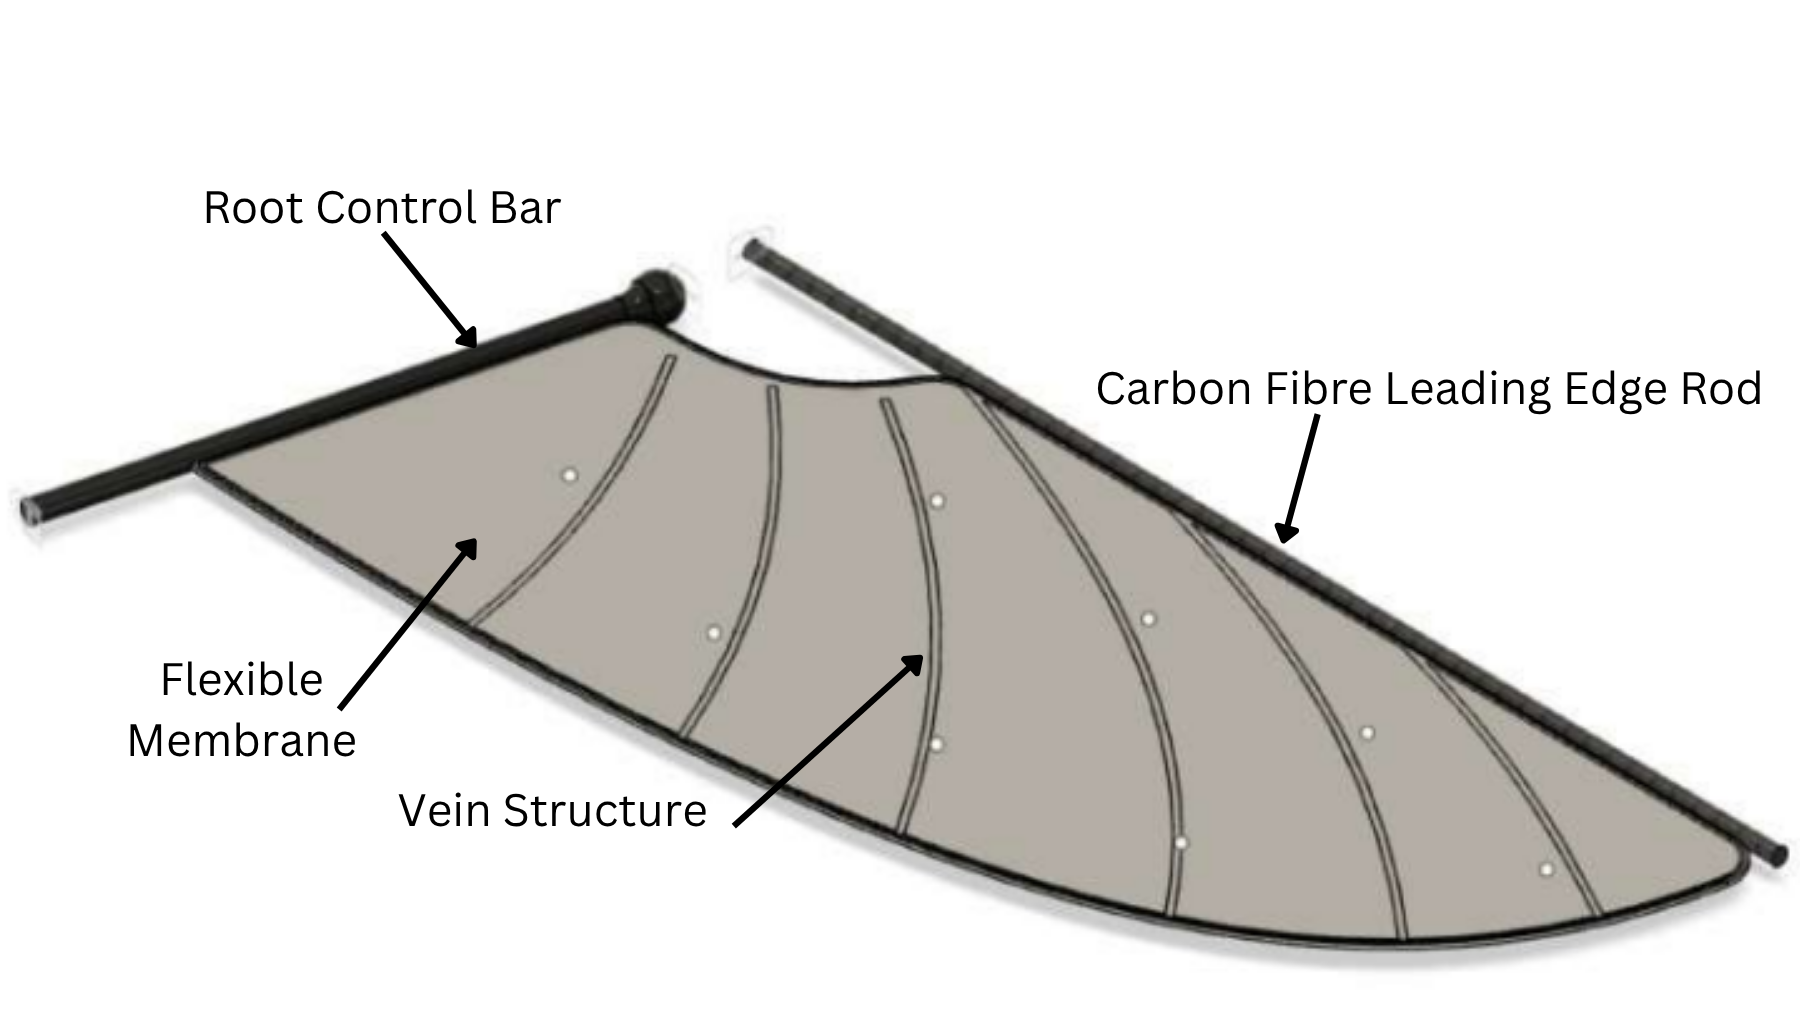
\includegraphics[height=4.5cm]{figures/baselinewingmodified.png}
    \caption{Baseline Wings: Final Wing Design from Previous Capstone Year \cite{MFWF_FinalReport2021}}
    \label{fig:baselinewingmodified}
\end{figure}

\subsection{Literature Review}

Building on insights from the 2021/22 and 2022/23 MFWF final reports~\cite{MFWF_FinalReport2021, MFWF_FinalReport2023}, a focused review of flapping-wing research was conducted to determine the deformation characteristics linked to efficient lift generation. The aim was to define an ``ideal'' deformation profile—specifically the combination of chordwise camber, passive twist, and spanwise bending observed in nature and flexible-wing FWMAVs. These characteristics directly inform the prototype designs developed this year. Figure \ref{fig:wingliftcharacteristics} shows important characteristics that contribute to a wings ability to generate lift. 

\begin{figure}[htb]
    \centering
    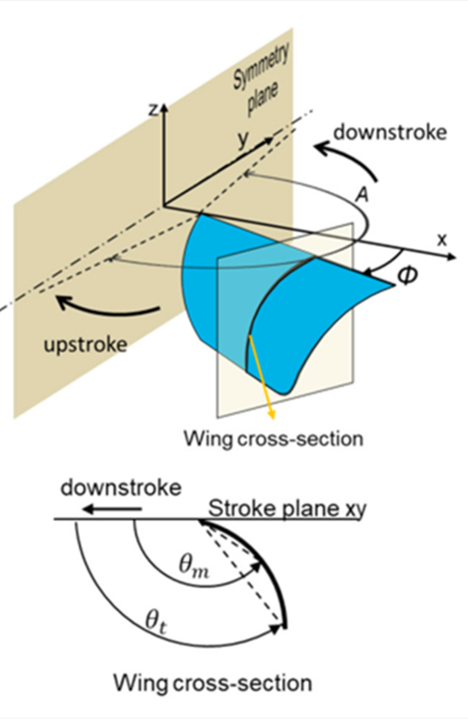
\includegraphics[height=6.5cm]{figures/wingliftcharacteristics.png}
    \caption{Wing Deformation Characteristics of a Flapping Wing \cite{dao2020corrugation}}
    \label{fig:wingliftcharacteristics}
\end{figure}

Most insect-scale flyers rely on passive aeroelastic deformation rather than rigid-wing aerodynamics\cite{ishihara}. Across beetles, flies, and insect-inspired robotic wings, three deformation modes consistently appear: camber, twist, and spanwise bending\cite{tian}. Chordwise camber between $5$--$12\%$ of chord was found to enhance the leading-edge vortex and increased lift during the power stroke\cite{wu}. Camber is evaluated using:
\begin{equation}
    f = \frac{h}{c},
\end{equation}
where $h$ is the maximum camber height and $c$ is the chord length. Thin membranes such as Mylar or polyurethane reliably achieve this camber range under aerodynamic loading.

Second, flexible wings typically exhibit $15^\circ$--$25^\circ$ of passive twist from root to tip~\cite{yoon,kraemer2012rapid}. The root follows the imposed motion while the tip lags due to lower torsional stiffness, shaping the leading edge vortex and improving downstroke lift. Third, insect wings bend downward by approximately $10$--$20\%$ of the semi-span under inertial loading~\cite{yoon}, aligning the wing with the local flow and reducing structural stress at flapping frequencies near 20--30 Hz.

Deformation also depends strongly on the interaction between veins and membrane stiffness~\cite{ishihara,kraemer2012rapid}. Intermediate veins help shape camber, a stiff leading edge maintains pitch at stroke reversal, and a compliant trailing edge supports both camber and twist.

\begin{table}[h]
\centering
\caption{Deformation characteristics for insect-scale flapping wings.}
\label{tab:ideal}
\begin{tabular}{l c l}
\hline
\textbf{Parameter} & \textbf{Target Range} & \textbf{Rationale} \\ \hline
Camber ratio $f = h/c$ & $5$--$12\%$ & Strong LEV and lift formation~\cite{wu,ishihara} \\
Passive twist & $15^\circ$--$25^\circ$ & Reduces tip stall; enhances downstroke lift~\cite{wu,kraemer2012rapid} \\
Spanwise bending & $10$--$20\%$ of semi-span & Aligns wing to flow; lowers stress~\cite{wu} \\
Membrane stiffness & Low--moderate & Allows smooth camber (Mylar, PP, PU) \\
Stiffness pattern & Stiff LE, flexible TE & Produces camber, twist, asymmetry~\cite{ishihara} \\ \hline
\end{tabular}
\end{table}

These deformation ranges define the criteria guiding this year's prototype development.It is important to note that these ranges are not idealized accross all flapping wings but specific wing architecture and geometries studied. Further experimentation will help identify an optimal range for the MFWF specifically based on flapping frequency, amplitude and lift force requirements. Variations in flexible membranes, vein geometry, and built-in camber were intentionally selected to evaluate how different structures reproduce these behaviours during the dynamic deflection tracking test.

\subsection{Design of Experiment}
A structured Design of Experiments (DOE) Table was developed to identify which wing architectures reproduce the similar deformation ranges established in the literature review. The DOE is fully defined, the baseline wing was remanufactured, an initial prototype set has been fabricated, and dynamic testing will proceed once the dynamic testing  setup is ready in the winter term. The objective is to determine how variations in membrane material and vein geometry influence camber, twist, and spanwise bending during flapping, while all other parameters remain same as in the baseline wing.

Following standard DOE principles, only a small set of variables are being varied, and all other conditions are held constant. The wings share a fixed span determined using the max span constraints mentioned earlier to ensure consistent inertial loading, while chord size, chord curvature, membrane choice, and vein geometry were selected as the experimental factors. This approach isolates the structural contributions of each design parameter, ensuring that observed differences in deformation can be attributed to controlled changes.

The prototypes span three built-in geometric camber levels (low, medium, high), implemented as camber angle extension to the membrane cutout, see Figure \ref{fig:camberangle}. 

\begin{figure}[htb]
    \centering
    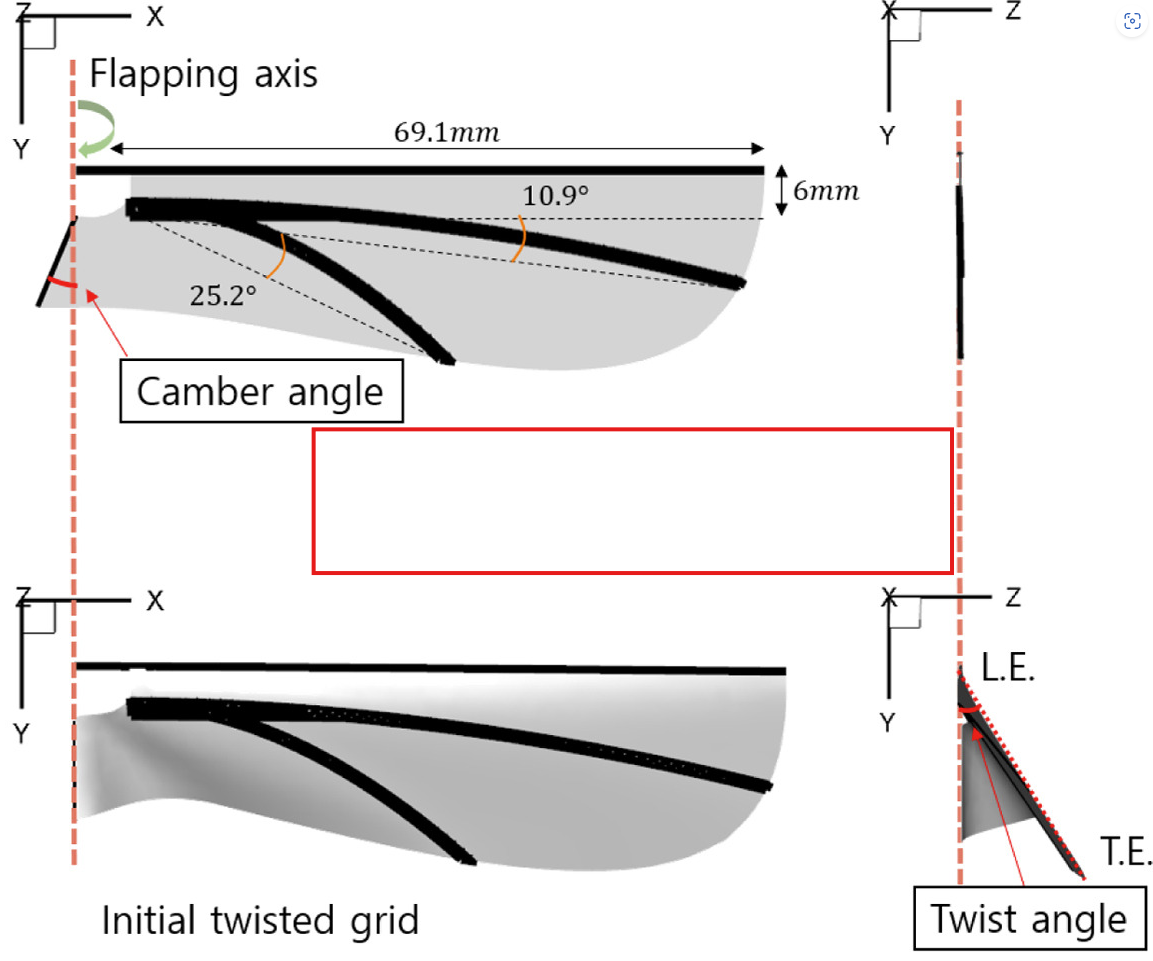
\includegraphics[height=6.5cm]{figures/camberangle.png}
    \caption{Camber Angle Extension and Twist Angle in Wing Design\cite{yoon}}
    \label{fig:camberangle}
\end{figure}

Membranes include polypropylene (PP) tape and Kapton, with Mylar included if available due to its favorable stiffness-to-weight properties. Vein geometry variations were introduced to shape chordwise flexibility and twist characteristics, including changes in vein stiffness and trailing-edge compliance.

All prototypes will undergo a dynamic deflection-tracking test and High-speed imaging will quantify deformation over the wingbeat cycle, including camber ratio and tip deflection as a measure of spanwise bending.

\begin{equation}
    f(t) = \frac{h(t)}{c},
\end{equation}
passive twist
\begin{equation}
    \theta_{\text{twist}}(t) = \theta_{\text{root}}(t) - \theta_{\text{tip}}(t),
\end{equation}

These quantities will be evaluated at mid-downstroke, stroke reversal, and mid-upstroke, allowing direct comparison to the ideal deformation targets reported for insect-scale wings.

The DOE provides a systematic and traceable framework for selecting the best-performing wing prototypes. Wings will be assessed on quantitative criteria: camber within $5$--$12\%$, twist between $15^\circ$ and $25^\circ$, spanwise bending within $10$--$20\%$ of the semi-span. A new wing variant with a modified leading-edge bar and control-bar geometry, introduced to meet the requirements of the electromagnetic flapping mechanism, will be evaluated under the same protocol. This experimental design ensures that the selected final wing is supported by measurable evidence and reflects the deformation behaviour of each wing prototype.

\begin{figure}[htb]
    \centering
    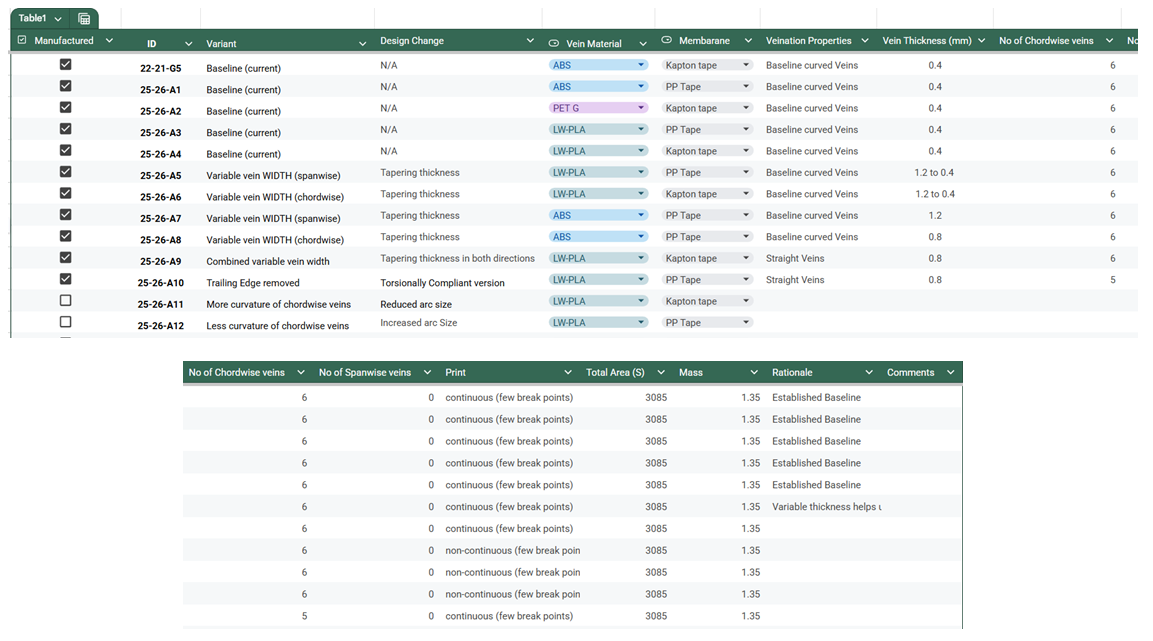
\includegraphics[height=9.5cm]{figures/doetable.png}
    \caption{Design of Experiments (Prototyping) Table }
    \label{fig:doetable}
\end{figure}
\subsection{Prototypes}
Prototyping this term focused on rebuilding a reliable set of baseline wings, and improving manufacturability. Since no testing has been conducted yet, all work centered on fabrication, refinement, and preparing the prototypes for testing. These tests will validate functionality of the prototypes

A major portion of the effort involved remanufacturing the baseline wing used in previous years. Early prints showed issues with vein thickness uniformity, and bubbles in the tape membrane. The baseline design was therefore modified to introduce curved edges, reprinted multiple times, with adjustments to print orientation, support strategy, and extrusion temperature. These changes resulted in improved prints.

\begin{figure}[htb]
    \centering
    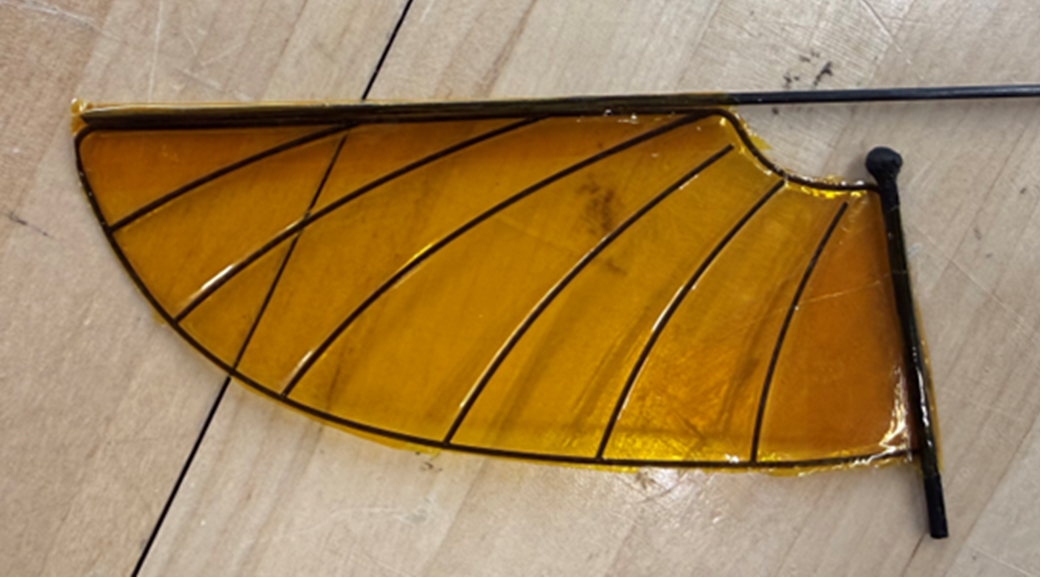
\includegraphics[height=4.5cm]{figures/newlymanufacturedwing.png}
    \caption{Baseline Wing Remanufactured with PETG Veins}
    \label{fig:newlymanufacturedwing}
\end{figure}

Beyond reproducing past work, the baseline geometry was also modified to improve fatigue resistance. Thin regions near the root and trailing edge experienced cracking during handling, indicating insufficient durability for prolonged dynamic motion. Local sharp internal corners were smoothed, and vein intersections were thickened slightly to distribute cyclic loads more evenly. These small geometric changes preserve the aeroelastic behaviour of the original design while significantly increasing the wing’s operational lifespan.

\begin{figure}[htb]
    \centering
    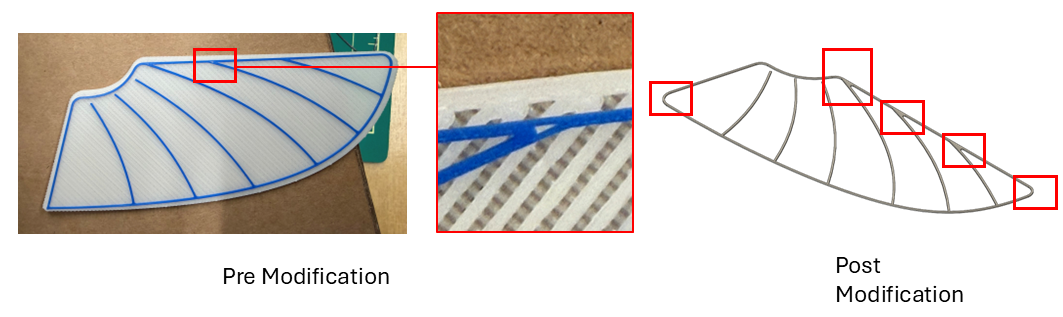
\includegraphics[height=4.5cm]{figures/baselinedesignchanges.png}
    \caption{Design Changes to Improve the Baseline Wing}
    \label{fig:baselinedesignchanges}
\end{figure}

A substantial amount of time went into resolving 3D-printing issues. LW-PLA required careful tuning to avoid voiding, layer delamination, and uncontrolled expansion. Several prints failed due to nozzle clogging, inconsistent extrusion, and instability when printing thin trailing edge veins for some prototypes. Adjustments included slowing down perimeter speeds, and increasing bed adhesion using custom brims. Printer calibration also had to be redone to correct some of these issues.

Once the baseline was manufactured successfully, attention shifted towards designing new wings that span the design variations outlined in the DOE. Multiple prototypes were fabricated with different chord sizes, built-in camber levels (low, medium, high), membrane materials (PP and Kapton), and vein geometries, see Figure \ref{fig:prototypes}. The 3D printed veins shown in Figure \ref{fig:prototypes} were not fully manufactured at the end of the term due to uncertainty in the interface between the the control bar and our test flapper, as the team is unsure what mechanism will be ready in time for the dynamic wing test. 

\begin{figure}[htb]
    \centering
    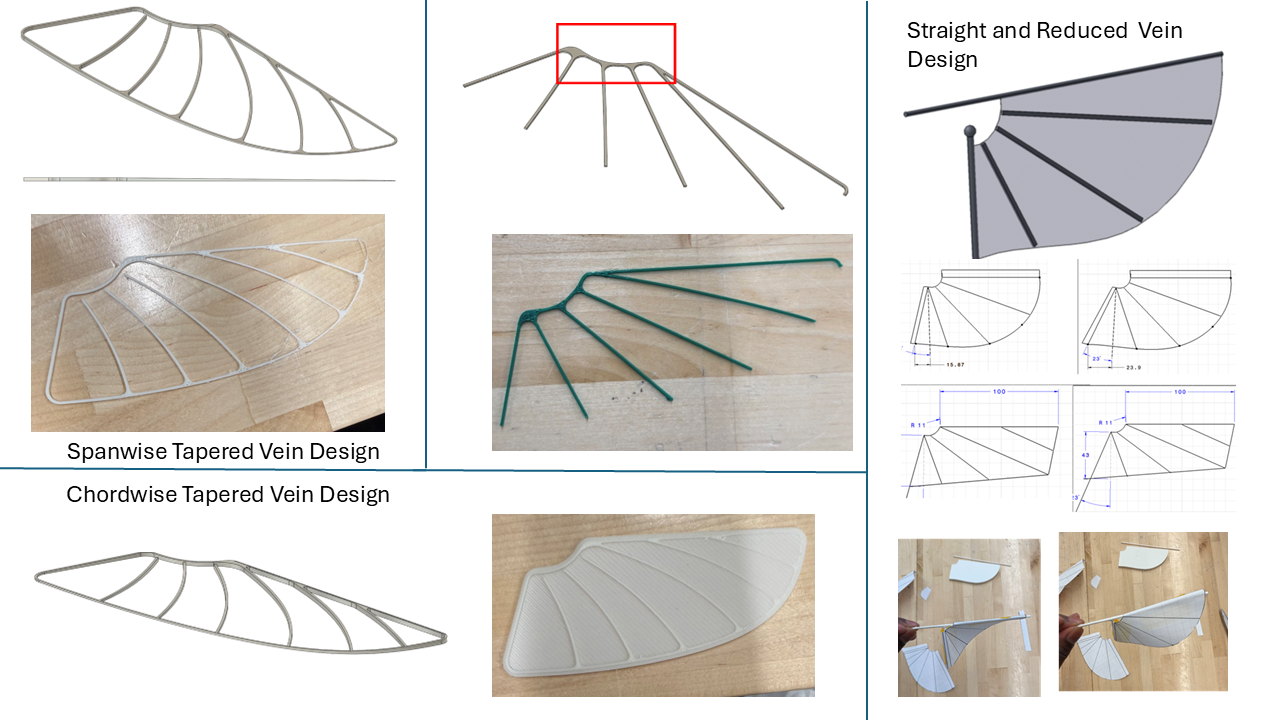
\includegraphics[height=6.5cm]{figures/prototypes.png}
    \caption{Design Changes to Improve the baseline Wing}
    \label{fig:prototypes}
\end{figure}

The final prototyping task involved modifying the leading-edge bar and control-bar design. This change was required after the decision to remove twist modulation by the electromagnetic flapping-mechanism team. Their system demands a different interface that can deliver the same stiffness near the root. The updated control bar and leading edge rod design improves load transfer into the wing, and ensures compatibility with the actuator’s stroke pattern. This modified bar will be used for all wings intended for dynamic testing next term. A more detailed version made of carbon fibre will be fabricated once interface decisions have been agreed on my the two teams during the winter term.

\begin{figure}[htb]
    \centering
    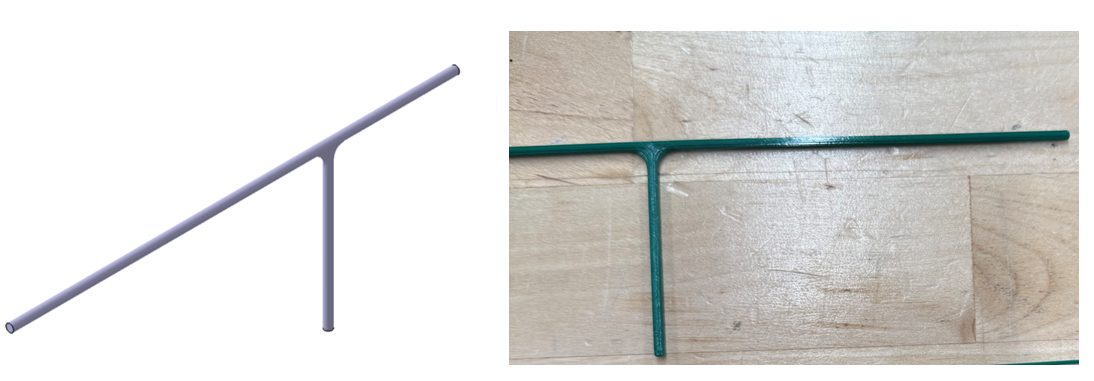
\includegraphics[height=4.5cm]{figures/controlbar.png}
    \caption{Preliminary Control Bar for testing}
    \label{fig:controlbar}
\end{figure}

\subsection{Plan for Winter Semester}
Work in the winter semester will focus on analysing the results from dynamic deflection-tracking tests and comparing the measured wing deformation to the ranges reported in the literature. From the high-speed recordings, quantitative metrics such as instantaneous camber ratio, root-to-tip twist, and spanwise bending amplitude will be extracted across multiple points in the flapping cycle. Additional timing data, such as phase lag between the leading edge and trailing edge, will help identify whether a wing responds too stiffly or too softly under dynamic loading. These measurements will directly inform the next round of prototypes by identifying which vein geometries or membrane materials produce desirable deformation patterns and which designs deviate from expected behaviour. Wings that demonstrate controlled camber formation, smooth passive twist, and repeatable bending profiles will be refined and re-printed for aerodynamic lift testing. 
In parallel, remaining interface questions with the electromagnetic flapping-mechanism team will be finalized to ensure that the revised leading-edge bar and control-bar designs integrate cleanly with their actuation system. Together, this work will establish a clear deformation-based selection pathway for the prototypes proceeding to aerodynamic evaluation.

\newpage
\section{Dynamic Testing and Motion Tracking}
\label{chap:Justin_Denneny}
\textbf{Student:} Justin Denneny
\subsection{Background}

The Micro Flapping Wing Flyer uses a flexible membrane wing, and the way this wing changes shape during motion plays a major role in how it behaves aerodynamically. Static testing alone cannot show this because the wing does not stay rigid when it flaps. Instead, it bends, lags, twists slightly, and responds to the forces acting on it. These dynamic effects are known to influence lift and overall performance, which has been shown in previous flapping wing research such as Lentink and Dickinson~\cite{Lentink2009}.

Since the previous capstone team already completed detailed static testing for the same wing geometries used this year, repeating that work during this semester would not have added new information. Because of this, my focus was on building the dynamic testing capability: creating a setup that allowed the wing to be flapped while being recorded clearly, and developing a MATLAB system that could track how the wing deformed throughout motion. This dynamic behaviour is needed so that we can eventually compare wings not just by stiffness, but by how they behave when actually moving. A calibration step was also introduced so the pixel motion could be converted into millimetres, allowing the deformation results to be expressed in physical units.
 
\subsection{Dynamic Testing Setup}

At the start of the semester, I tested several different ways to record the wing. The biggest issue early on was getting clean footage that the tracking algorithm could work with. The membrane surface reflects light easily, so small changes in angle or lighting caused glare or shadows that made the markers hard to detect. Some backgrounds blended with the wing, and different camera heights caused distortion.

After multiple trials with different lighting, backgrounds, and phone positions, the setup that worked best used an overhead camera looking straight down onto a white background. The white surface removed most of the clutter and shadows and made the markers stand out clearly. The top-down view also ensured that the wing appeared as a clean 2D projection, which is important since the tracking script measures pixel displacement frame by frame. This layout was stable and gave the most consistent detection results throughout the semester. This setup is now fully repeatable for all future wing prototypes and will be used as the standard configuration for the dynamic database.
 
\begin{figure}[htb]

    \centering

    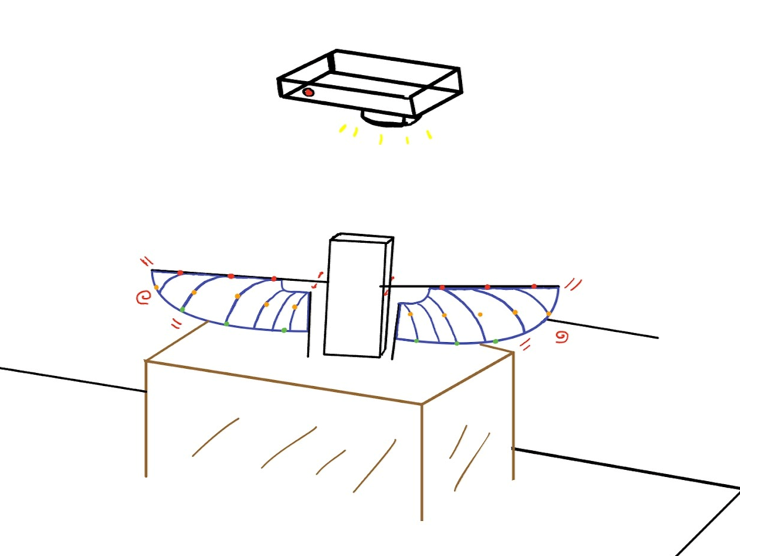
\includegraphics[height = 6.5cm]{figures/Dynamic Testing Setup.png}

    \caption{Dynamic Test Setup}

    \label{fig:dynamic_setup}

\end{figure}
 
\subsection{Marker Placement}
To measure how the wing bends while flapping, I applied three coloured markers along the span. A green marker was placed at the root, a red marker at the mid span rib, and a blue marker at the wing tip. These points were selected because they represent three key structural locations. The root gives information on how much the mount shifts or flexes, the mid span shows how the membrane bends during motion, and the tip experiences the greatest displacement.

This style of marker placement is also used in insect wing studies where researchers track a few points to understand bending patterns~\cite{Bomphrey2010}.
 
\begin{figure}[htb]

    \centering

    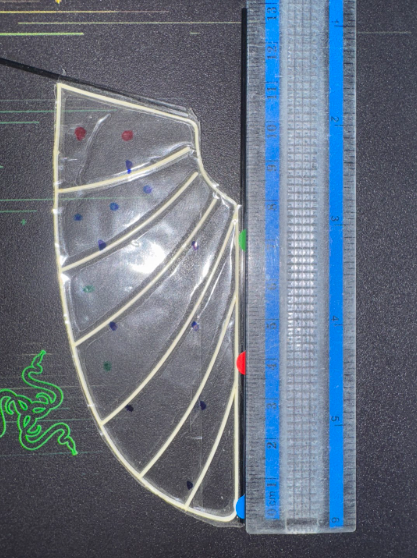
\includegraphics[height = 6.5cm]{figures/Wing w Test Markers.png}

    \caption{Wing with Marker Placement.}

    \label{fig:marker_placement}

\end{figure}
 
\subsection{Motion Tracking Development}

With the physical setup established, the next objective was to develop a MATLAB-based tracking pipeline. Each recorded video was processed frame by frame, converted from RGB to HSV colour space, and segmented using tuned thresholds for each marker colour. HSV segmentation was chosen because it is better to ambient lighting variation, improving detection consistency. For every frame, the centroid of each detected colour region was extracted. Missing detections were interpolated and small frame-to-frame jitter was smoothed to produce continuous trajectories.
 
Beyond producing numerical outputs, the system generated an overlay video displaying the original footage with tracked marker positions and their motion paths superimposed. This provided immediate visual confirmation that the segmentation and tracking were functioning correctly. If the overlay accurately matched the motion of the physical markers, the extracted data was considered valid. Figure~\ref{fig:tracking_overlay} shows an example frame from one of these overlay videos.
 
\begin{figure}[htb]

    \centering

    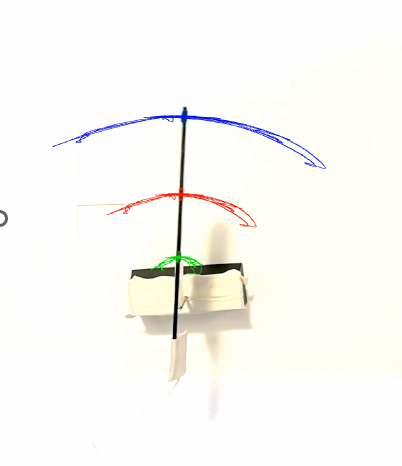
\includegraphics[height = 6.5cm]{figures/MATLAB Generated Wing Tracking Overlay.png}

    \caption{MATLAB Motion Marker Tracking}

    \label{fig:tracking_overlay}

\end{figure}
 
This pipeline now provides deflection histories, calibrated displacement values, trajectories, phase relationships, and spanwise bending shapes, forming the foundation for dynamic comparison between wing geometries. The code was written in a modular way so new wing designs, marker layouts, or additional metrics can be added without rewriting the entire pipeline.
 
\subsection{Preliminary Dynamic Results}

To test the system, several videos were recorded using manually induced flapping. Although the motion was not perfectly smooth or repeatable, it was still useful for checking how well the tracking worked. The tracking was able to follow all three markers throughout the test.

The vertical displacement measured at the root, mid span, and tip is shown in Figure~\ref{fig:tracking_overlay}. The results matched what would be expected for a flexible membrane wing. The tip experienced the largest deflection, the mid span produced a smoother and smaller response, and the root moved only slightly. This behaviour is consistent with bending patterns described in flexible wing literature, such as Shyy et al.~\cite{Shyy2013}.
 
\begin{figure}[htb]

    \centering

    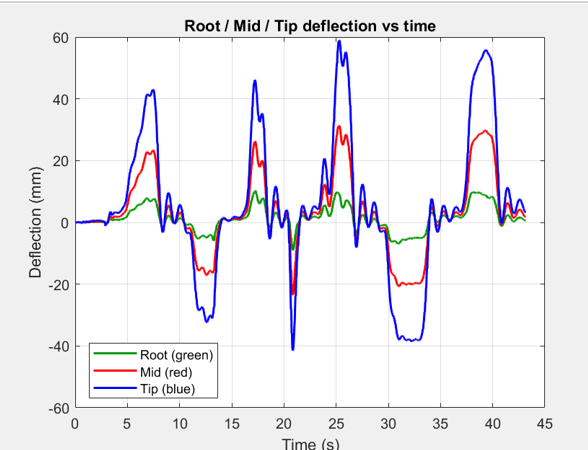
\includegraphics[height = 6.5cm]{figures/Preliminary Wing Deflection.png}

    \caption{Preliminary Vertical Deflection for Manual Flapping}

    \label{fig:dyn_deflection}

\end{figure}
 
In addition to the time based deflection data, I extracted a spanwise deformation shape from the tracked points. This shows the shape of the wing along its span at the moment of maximum tip displacement. The result showed the root nearly stationary, a smooth bending curve through the mid span, and the tip at the largest displacement. This resembles a first mode bending shape and helps compare wings under the same conditions. Being able to extract a mode shape also provides a starting point for linking wing flexibility to aerodynamic behaviour, such as how deformation might influence lift.

 
\begin{figure}[htb]

    \centering

    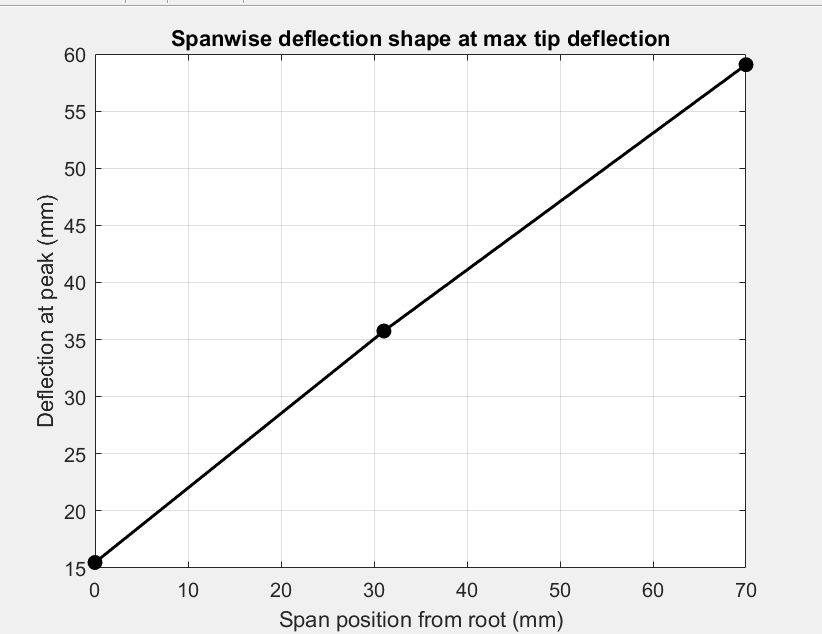
\includegraphics[height = 6.5cm]{figures/Spanwise Deflection Shape.png}

    \caption{Spanwise Deflection - Mode Shape}

    \label{fig:mode_shape}

\end{figure}
 
These results show that the motion tracking system works consistently and that most irregularities came from the manual flapping, not the algorithm. Cleaner and more repeatable data is expected once a motor based flapping system is introduced. Once the servo-driven flapping mechanism is implemented, additional metrics such as dominant flapping frequency, phase lag, and tip velocity will be incorporated into the testing database.
 
\subsection{Use of Previous Static Testing Data}

At the beginning of the term, the static testing results from the previous capstone year were reviewed. Because the wing geometries tested this semester were identical to those previously evaluated, their static stiffness characteristics remain valid. Repeating those tests would not have produced meaningful new insights. This allowed the focus this semester to remain entirely on developing the dynamic testing and motion-tracking framework. Static testing will resume next semester once new wing designs are fabricated so that static and dynamic properties can be documented consistently across all geometries.
 
\subsection{Plan for Winter Semester}

The primary objective for Winter 2026 is to transition from manual excitation to a fully controlled servo-driven flapping mechanism capable of producing consistent, repeatable motion. This will allow precise measurement of dynamic stiffness, deformation patterns, and frequency response. The wing root will be rigidly mounted to eliminate drift observed during preliminary tests. Once new wing geometries are fabricated, each will undergo both static and dynamic characterization. Key parameters such as peak deflection, dominant frequency, phase lag, and spanwise mode shape will be extracted and compiled into a dynamic testing database parallel to the existing static database.
 
A long-term goal is to investigate whether dynamic deformation data can be used to estimate aerodynamic performance, including approximate lift generation. Metrics such as wingtip velocity, instantaneous curvature, and effective angle of attack may be combined with simplified aerodynamic models to infer lift trends. If successful, the dynamic testing platform will provide both structural and aerodynamic insight, strengthening the wing selection process for the Micro Flapping Wing Flyer.
 
